\svnid{$Id$}
\chapter{Nitric Oxide Reduction in \Nm{}}
\label{chap:noreduction}
\section{Aerobic Nitric Oxide Reduction}
\subsection{Introduction}
The next dataset used in the iterative approach to parameter estimation was of aerobic oxygen reduction interrupted by the addition of Nitric Oxide. These datasets are the next most complicated after aerobic oxygen reduction as it introduces the nitric oxide reduction pathway. In this case the oxygen reduction and Nitric Oxide reduction pathways are active. Additionally, inactivation of \cbbthree{} by Nitric Oxide was occurring. The portions of the ETC relating to Nitric Oxide reduction are shown graphically in Figure \ref{fig:no_resp_chain}. However this pathway cannot be isolated \textit{in vivo} as \Nm{} is incapable of completely anaerobic respiration therefore the required parts of the model are actually those from Chapter \ref{chap:oxygenreduction} and those in Figure \ref{fig:no_resp_chain}.
\begin{figure}[tbp]
  \centering
    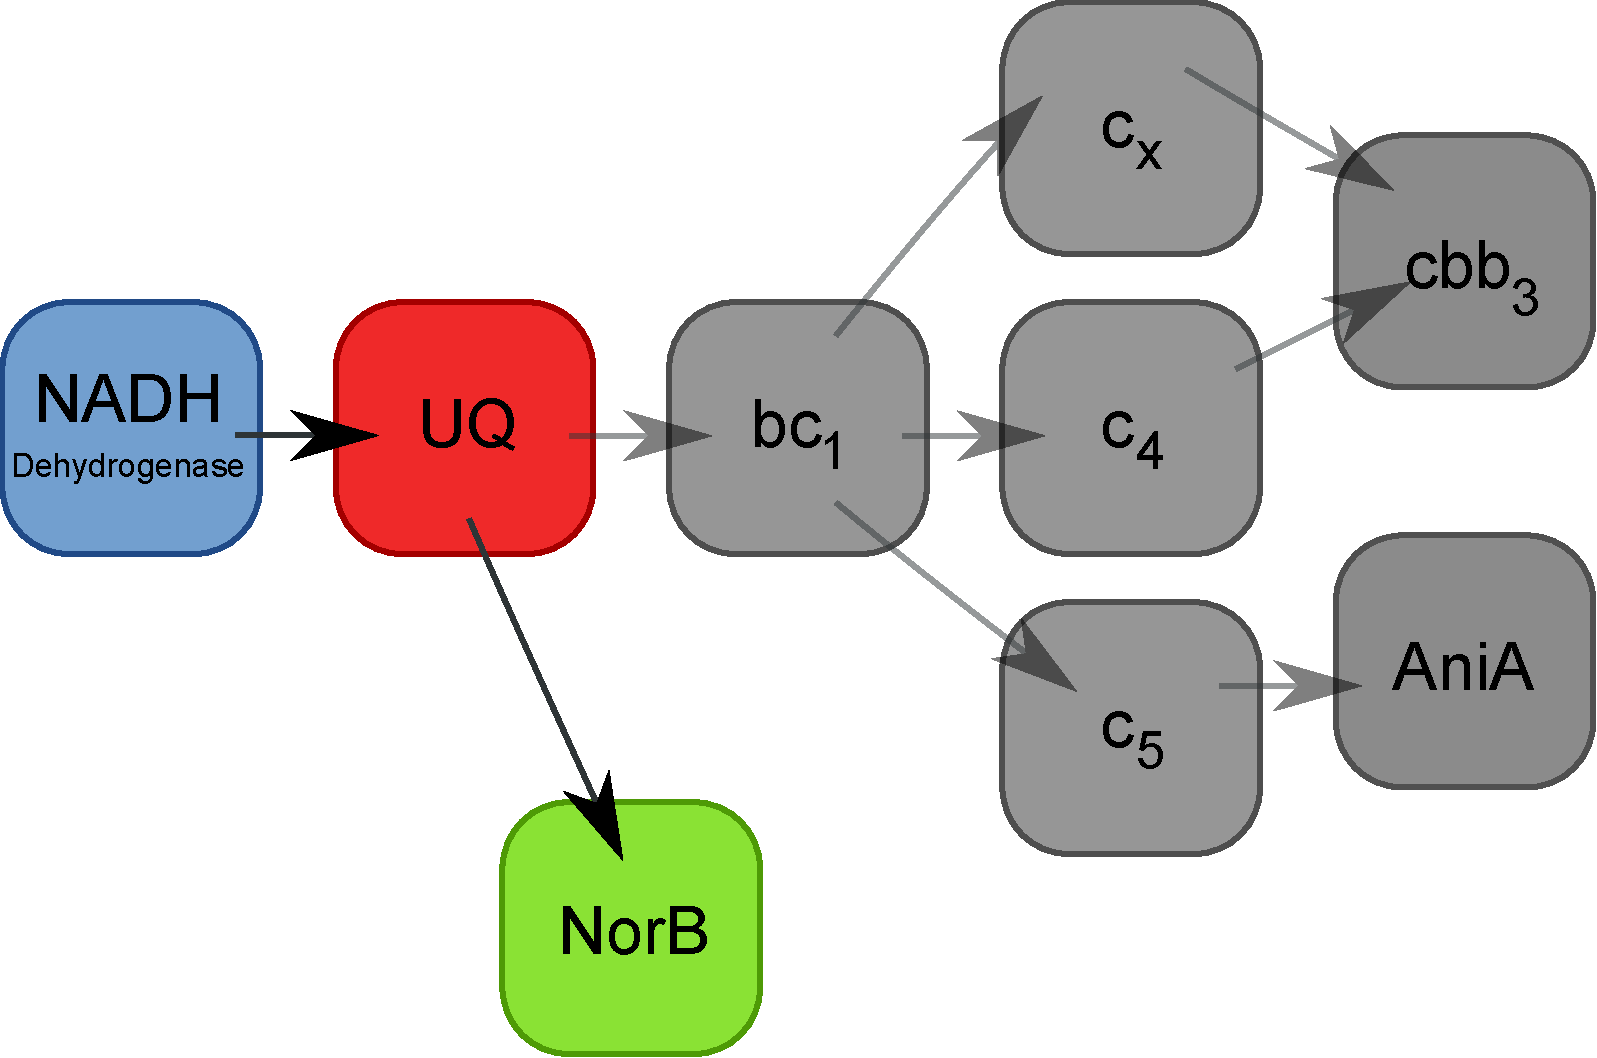
\includegraphics[width=14cm]{06-noreduction/data/no_resp_chain.pdf}
    \caption[Nitric oxide reducing electron transport chain of \Nm{}]{{\bf Nitric oxide reducing electron transport chain of \Nm{}.} This shows the complete electron transport chain of \Nsm{} with the components irrelevant to nitric oxide reduction greyed out.
  \label{fig:no_resp_chain}}
\end{figure}\\
The equations that describe this portion of the ETC are:
\begin{eqnarray*}
\frac{d[O_2]}{dt} & = & \beta(1-[O_2]/K_O) - k_{1}[C_a][O_2]\\
\frac{d[Q_a]}{dt} & = & g([Q] - [Q_a]) - l_3[Q_a]([B] - [B_a]) - f[Q_a]([X]-[X_a])\\
\frac{d[X_a]}{dt} & = & -k_3([C] - [C_a] - [C_X])[X_a]  - m_3([A] - [A_a])[X_a] + f[Q_a]([X]-[X_a])\\
\frac{d[C_a]}{dt} & = & k_3([C] - [C_a] - [C_X])[X_a] - k_{1}[C_a][O_2] - k_5[C_a][NO] + k_6[C_X]\\
\frac{d[NO]}{dt} & = & m_{1}[NO_2^-][A_a] - l_1[NO][B_a] - k_5[C_a][NO] + k_6 [C_X] - \gamma[NO]\\
\frac{d[C_X]}{dt} & = & k_5[C_a][NO] - k_6 [C_X]\\
\frac{d[B_a]}{dt} & = & l_3[Q_a]([B] - [B_a]) - l_1[NO][B_a]
\end{eqnarray*}
These equations describe the change in concentration of Nitric Oxide over time, which is the experimentally observable value (in addition to the afore modelled oxygen). Also being modelled was the change in concentration of inhibited \cbbthree{} and the reduction state of NorB. This more complete portion of the model involved 24 parameters and variables which were to be estimated. This number includes the 13 values already estimated in Chapter \ref{chap:oxygenreduction}.
\subsection{Experimental Results}
Generation of Nitric Oxide reduction datasets required the growth of MC58 (wild type \Nsm{}) in aerobic conditions until mid log-phase growth had been achieved. This corresponds to an $OD_{600}$ of 0.3-0.9 and usually required an incubation period of roughly 3 hours. Once the required cell density had been obtained, the culture was transferred to the oxygen electrode chamber and the oxygen and nitric oxide concentrations recorded as the culture respired. To model nitric oxide reduction required that nitric oxide solution was added to the culture while it is respiring aerobically. Part-way through aerobic respiration nitric oxide solution was added to various final concentrations all at $\approx 5~\mu$M and the culture then left to reduce nitric oxide (in addition to oxygen). The nitric oxide reduction datasets generated and used for parametrisation of this portion of the model are shown in Figures \ref{fig:nodata}, \ref{fig:nodata2}, \ref{fig:nodata1} \& \ref{fig:nodata3}. Unfortunately the experimental data upon addition of nitric oxide is very difficult to reliably reproduce, with different cultures having apparently different tolerances to nitric oxide (data not shown).

%ds1
\begin{figure}[tbp]
 \centering
 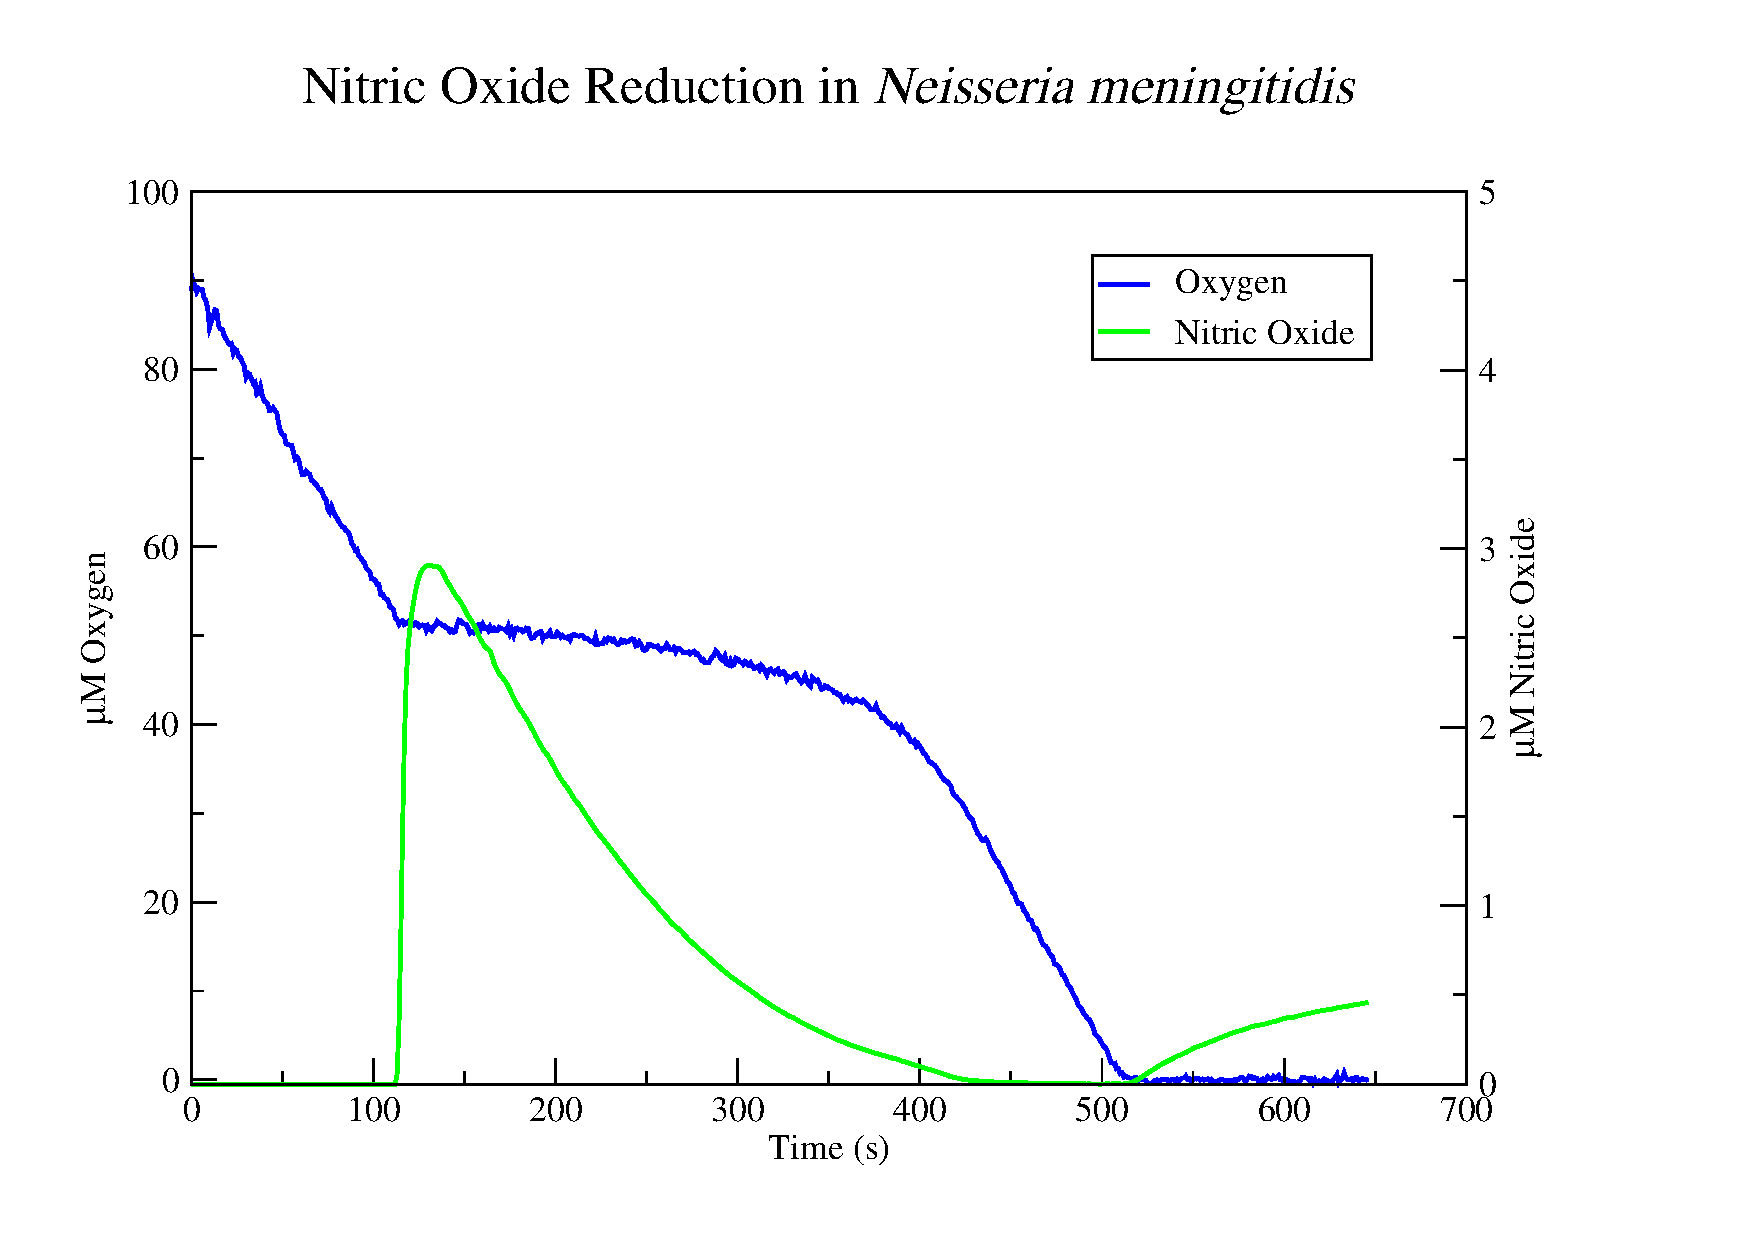
\includegraphics[height=10cm, trim=1cm 1cm 3cm 1cm, clip=true]{./06-noreduction/data/aer-no-data.pdf}
 % nosim.eps: 0x0 pixel, 300dpi, 0.00x0.00 cm, bb=0 0 794 595
 \caption[{Nitric Oxide Reduction in \textit{Neisseria meningitidis}.}]{{\bf Nitric Oxide Reduction in \textit{Neisseria meningitidis}.} This dataset shows the effect on rate of oxygen reduction as nitric oxide (to $\approx 3~\mu M$) is introduced to the respiring system which also appears to have been partially primed for nitric oxide reduction. Note that the increase in nitric oxide concentration seen at the end of the dataset is most likely due to drift in the electrode.}
 \label{fig:nodata}
\end{figure}
The dataset in Figure \ref{fig:nodata} appears to show a system that was partially primed for microaerobic respiration. In this case it was speculated that there was a small amount of NorB (nitric oxide reductase) present. Initially the oxygen reduction was carried out in exactly the same manner as in Chapter \ref{chap:oxygenreduction}. Upon addition of nitric oxide, oxygen respiration slowed and almost stopped as a result of competition for electrons between \cbbthree{} and NorB, and the direct chemical inhibition of \cbbthree{} by NO. Nitric oxide started to be removed as a combination of diffusion (although this rate will be low as shown in the previous two datasets) and reduction via NorB. Once the NO has been removed from the system oxygen reduction resumes at almost the same rate as before and still has the same high affinity feature as the oxygen reduction datasets in Chapter \ref{chap:oxygenreduction}.

%ds2
\begin{figure}[tbp]
 \centering
 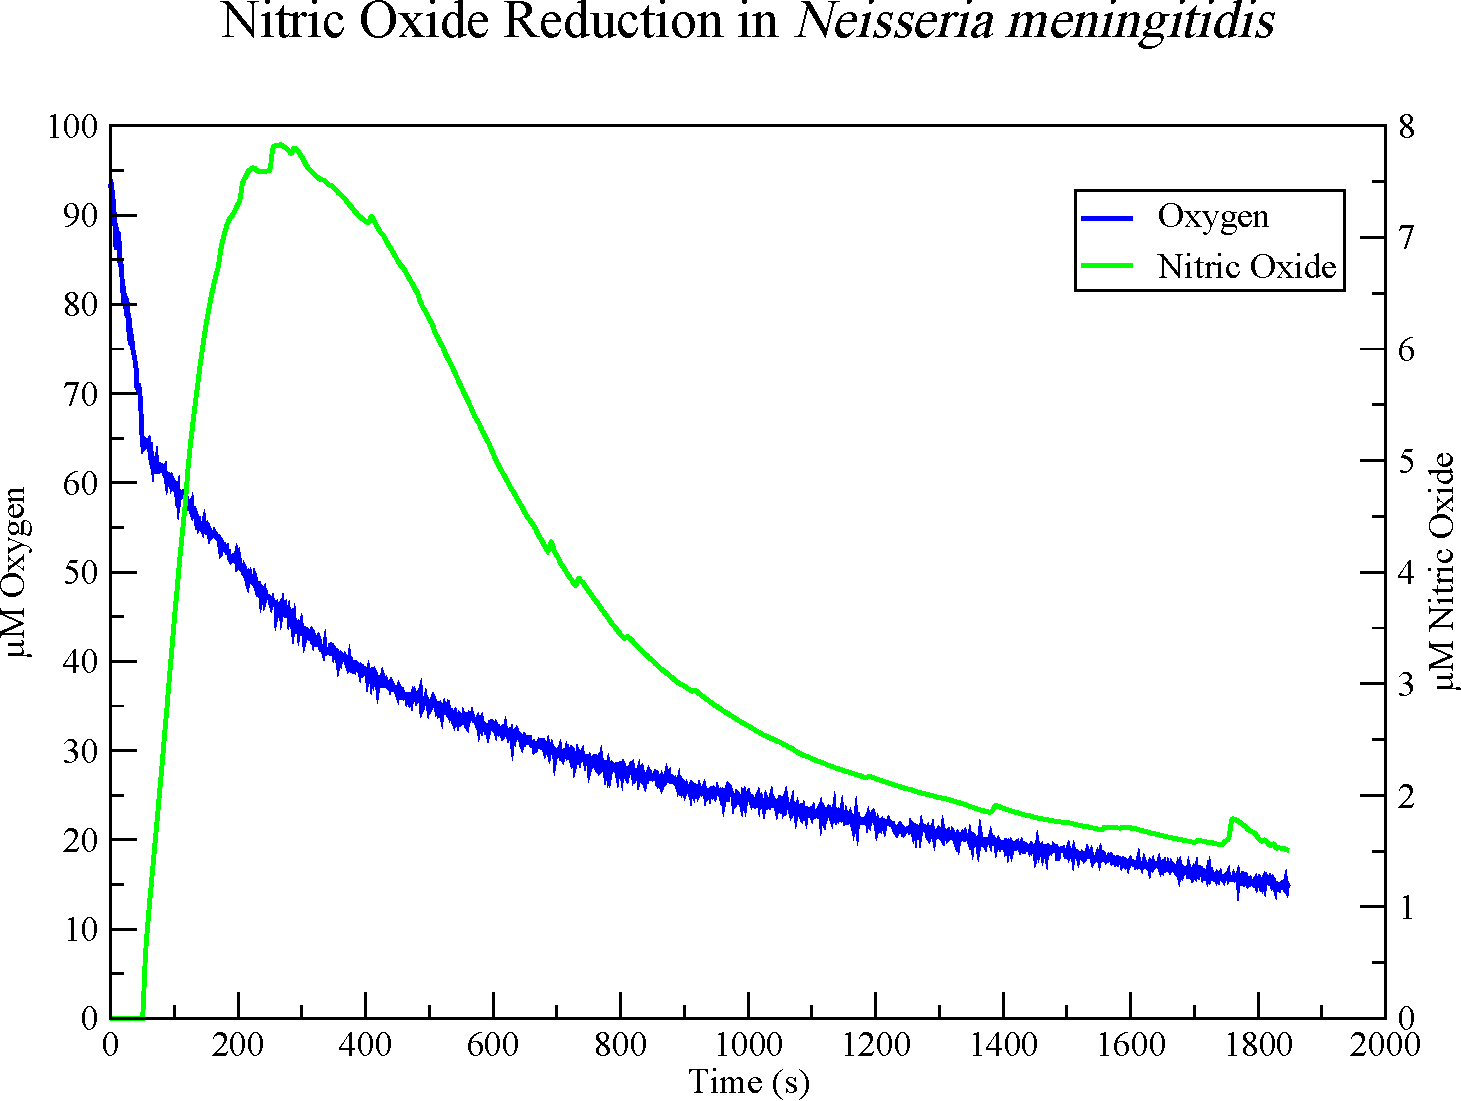
\includegraphics[height=10cm, trim=1cm 1cm 3cm 1cm, clip=true]{./06-noreduction/data/aer-no-data2.pdf}
 % nosim.eps: 0x0 pixel, 300dpi, 0.00x0.00 cm, bb=0 0 794 595
 \caption[{Nitric Oxide Reduction in \textit{Neisseria meningitidis}.}]{{\bf Nitric Oxide Reduction in \textit{Neisseria meningitidis}.} This dataset shows the effect on rate of oxygen reduction as a larger amount of nitric oxide (to $\approx 7.8~\mu M$) is introduced to the respiring system.}
 \label{fig:nodata2}
\end{figure}
The dataset in Figure \ref{fig:nodata2} shows a larger change in the rate of oxygen reduction than that of Figure \ref{fig:nodata1} when a larger amount of nitric oxide is introduced. Again the removal of nitric oxide will primarily be due to diffusion, although now at higher concentrations more nitric oxide will interact with \cbbthree{} temporarily inhibiting it. This inhibition causes the reduction in oxidase activity, and the sequestering of NO by \cbbthree{} also causes some of the visible reduction in nitric oxide concentration. The time-scale over which the nitric oxide disappears strongly suggests that it is not due to nitric oxide reductase activity. It may also be possible that at this concentration of nitric oxide some \cbbthree{} may have been permanently inhibited as mentioned in Chapters \ref{chap:intro} \& \ref{chap:model}. As the cultures in this dataset were obviously being negatively affected by the addition of such a high concentration of nitric oxide, either by permanent inhibition of \cbbthree{} or actual cell death, it was unlikely that this particular dataset could be used to accurately predict parameters in the model as it includes factors that were never part of the original model.

%ds3
\begin{figure}[tbp]
 \centering
 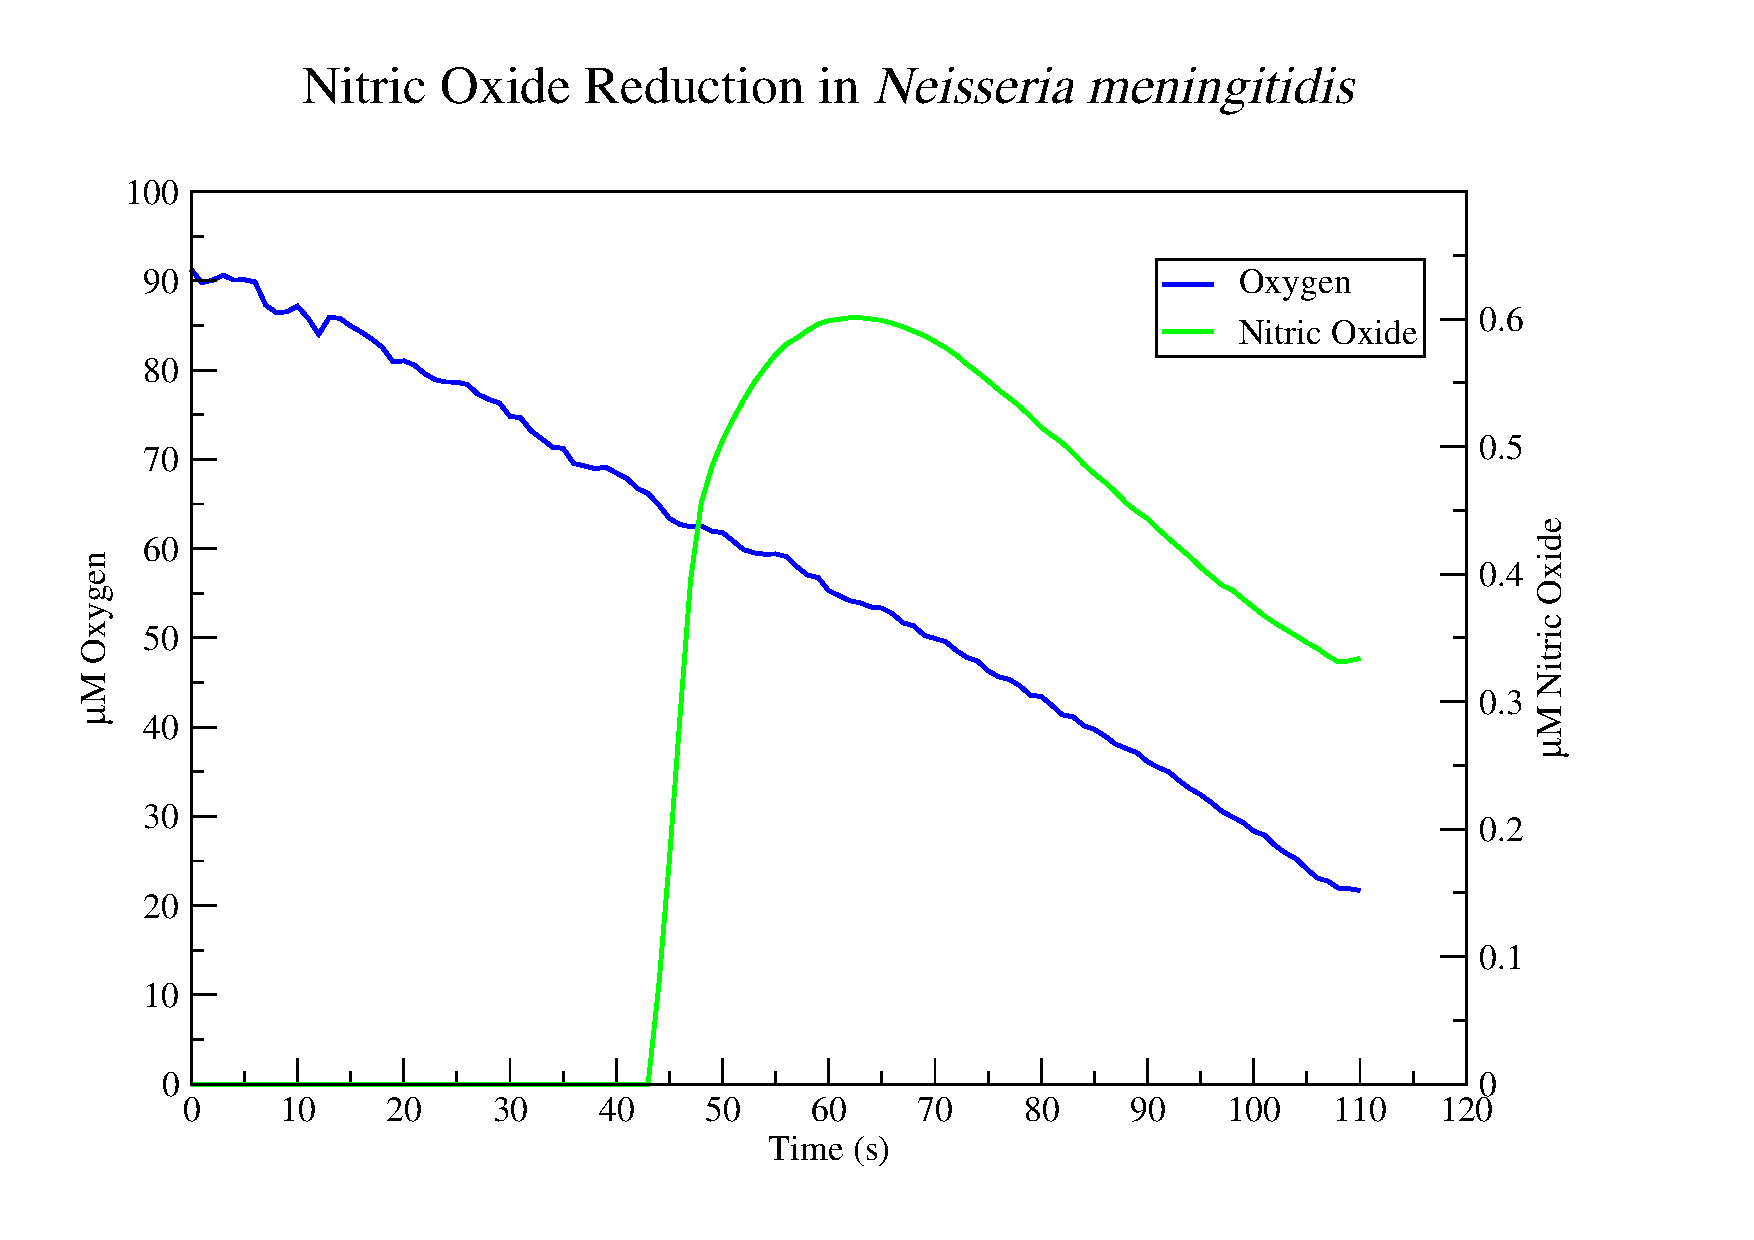
\includegraphics[height=10cm, trim=1cm 1cm 3cm 1cm, clip=true]{./06-noreduction/data/aer-no-data1.pdf}
 % nosim.eps: 0x0 pixel, 300dpi, 0.00x0.00 cm, bb=0 0 794 595
 \caption[{Nitric Oxide Reduction in \textit{Neisseria meningitidis}.}]{{\bf Nitric Oxide Reduction in \textit{Neisseria meningitidis}.} This dataset shows the effect on rate of oxygen reduction as a small amount of nitric oxide (to $\approx 0.6~\mu M$) is introduced to the respiring system.}
 \label{fig:nodata1}
\end{figure}
The dataset in Figure \ref{fig:nodata1} shows very little visible change in the rate of oxygen reduction when a small amount of nitric oxide is added. In actual fact the change in rate was an $\approx 3\%$ reduction after addition of nitric oxide based on linear regression of pre- and post-addition rates. The observed removal of nitric oxide is due primarily to diffusion, although there may also be some preliminary (as the culture has not been primed with nitric oxide) nitric oxide reductase activity. However for modelling purposes it was assumed that the nitric oxide reductase activity for this dataset is zero.

\begin{figure}[tbp]
 \centering
 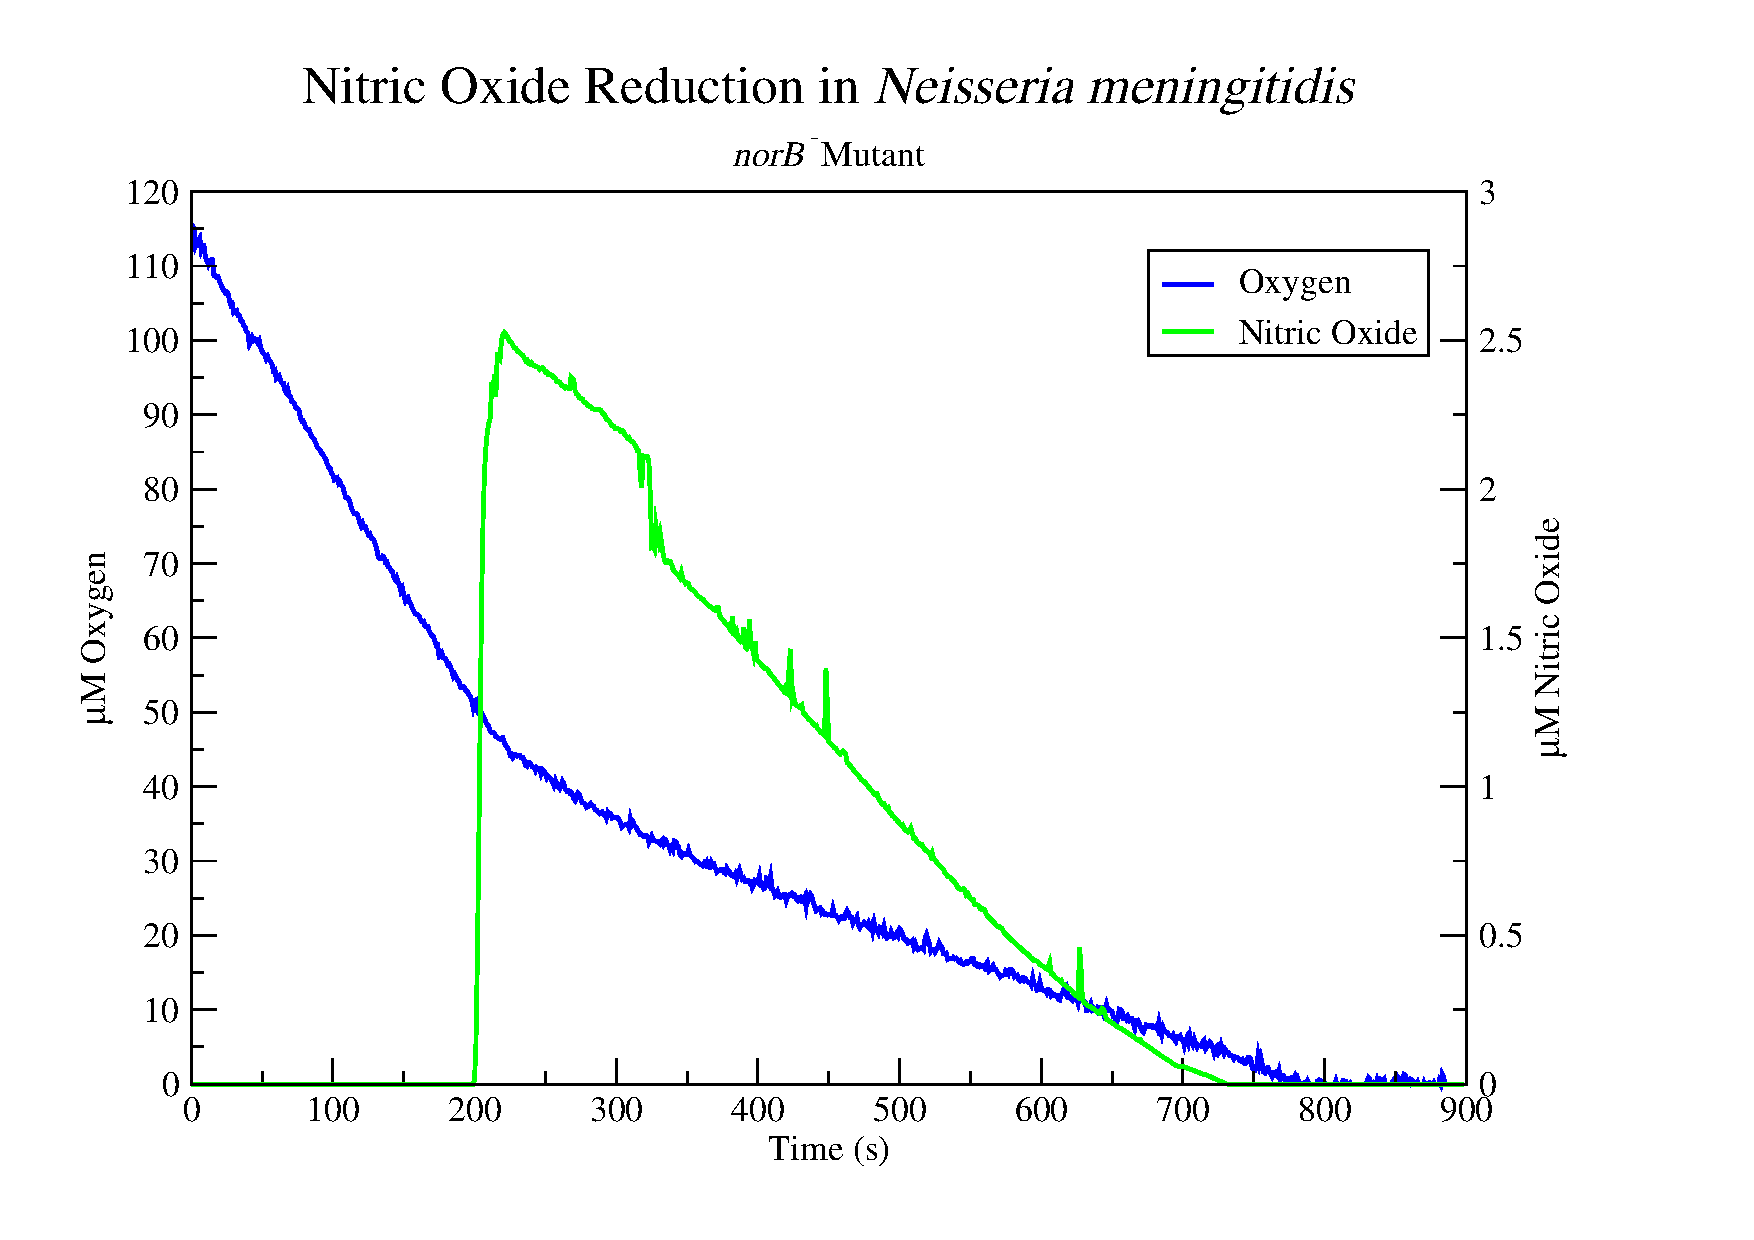
\includegraphics[height=10cm, trim=1cm 1cm 3cm 1cm, clip=true]{./06-noreduction/data/aer-no-data3.pdf}
 % nosim.eps: 0x0 pixel, 300dpi, 0.00x0.00 cm, bb=0 0 794 595
 \caption[{Nitric Oxide Reduction in \textit{Neisseria meningitidis}.}]{{\bf Nitric Oxide Reduction in \textit{Neisseria meningitidis}.} This dataset shows the effect on rate of oxygen reduction as nitric oxide (to $\approx 2.5~\mu M$) is introduced to a respiring $norB-$ mutant culture. Any removal of nitric oxide here is due to diffusion and sequestering by \cbbthree{} alone.}
 \label{fig:nodata3}
\end{figure}
The dataset in Figure \ref{fig:nodata3} shows a visible change in reduction rate of \cbbthree{} upon addition of nitric oxide. This is due to inhibition of the \cbbthree{} directly by nitric oxide. This culture is incapable of reducing nitric oxide, having a $norB^-$ mutation, thus the only route for removal of nitric oxide is by simple diffusion.

\subsubsection{Prior Probability Distributions}
As in Chapter \ref{chap:oxygenreduction} the integrative scheme requires that all the parameters involved have associated prior probability distributions. The posterior probability distributions from Chapter \ref{chap:oxygenreduction} were used as prior probability distributions in this chapter. Where new parameters were introduced (which had not been modelled thus far), the distributions were generated based upon published literature values which are noted in Chapter \ref{chap:model}. When using literature values the prior probability distributions were generated according to the same scheme as in Chapter \ref{chap:oxygenreduction}. Where the posterior probability distributions from Chapter \ref{chap:oxygenreduction} describe rate constants the raw values from the distributions were used as priors in this chapter. Where the distributions describe component concentrations, idealised lognormal distributions were used instead of the raw data to account for differing concentrations between cultures. The distribution of the parameter $\gamma$ - the rate of loss of NO - was initially assumed to be similar to $\beta$, thus the same probability distribution was used. For the other new parameters, lognormal distributions were used as priors as described in Chapter \ref{chap:oxygenreduction}. The values required to create idealised lognormal probability distributions for each parameter are shown in Table \ref{tab:noProbstat1}.

\begin{table}[ht]%needs to be 'here' as section is short
\renewcommand{\arraystretch}{1.5}
\begin{center}
\begin{tabular}{cccc|cccc}
\toprule
\textbf{Parameter} && ${\bar{x}}$ & $\sigma$ & \textbf{Parameter} && ${\bar{x}}$ & $\sigma$\\
\midrule
$k_1$ && 413.228 & 30.046 & g && 0.889 & 0.089\\
$k_3$ && 4.496 & 0.463 & f && 8.707 & 1.35\\
$l_1$ && 6 & 2 & $\gamma$ && 0.00014 & $4.67\times 10^{-6}$\\
$l_3$ && 1 & 2 & Q && 3.143 & 0.240\\
$k_5$ && 100 & 10 & X && 4.732 & 6.707\\
$k_6$ && 38 & 8 & B && 0.043 & 0.044\\
$\beta$ && 0.00014 & $4.67\times 10^{-6}$ & C && 0.043 & 0.044\\
\bottomrule
\end{tabular}
\end{center}
\caption[Prior Probability Table]{{\bf Prior Probability Table} This table shows the prior means and standard deviations used to create lognormal distributions to be used as the prior probability distributions.
\label{tab:noProbstat1}}
\end{table}
\afterpage{\clearpage}
The initial probability distributions used to start the Monte-Carlo runs are shown in Figure \ref{fig:aer_no_priors}.
\begin{figure}[tbp]
 \centering
 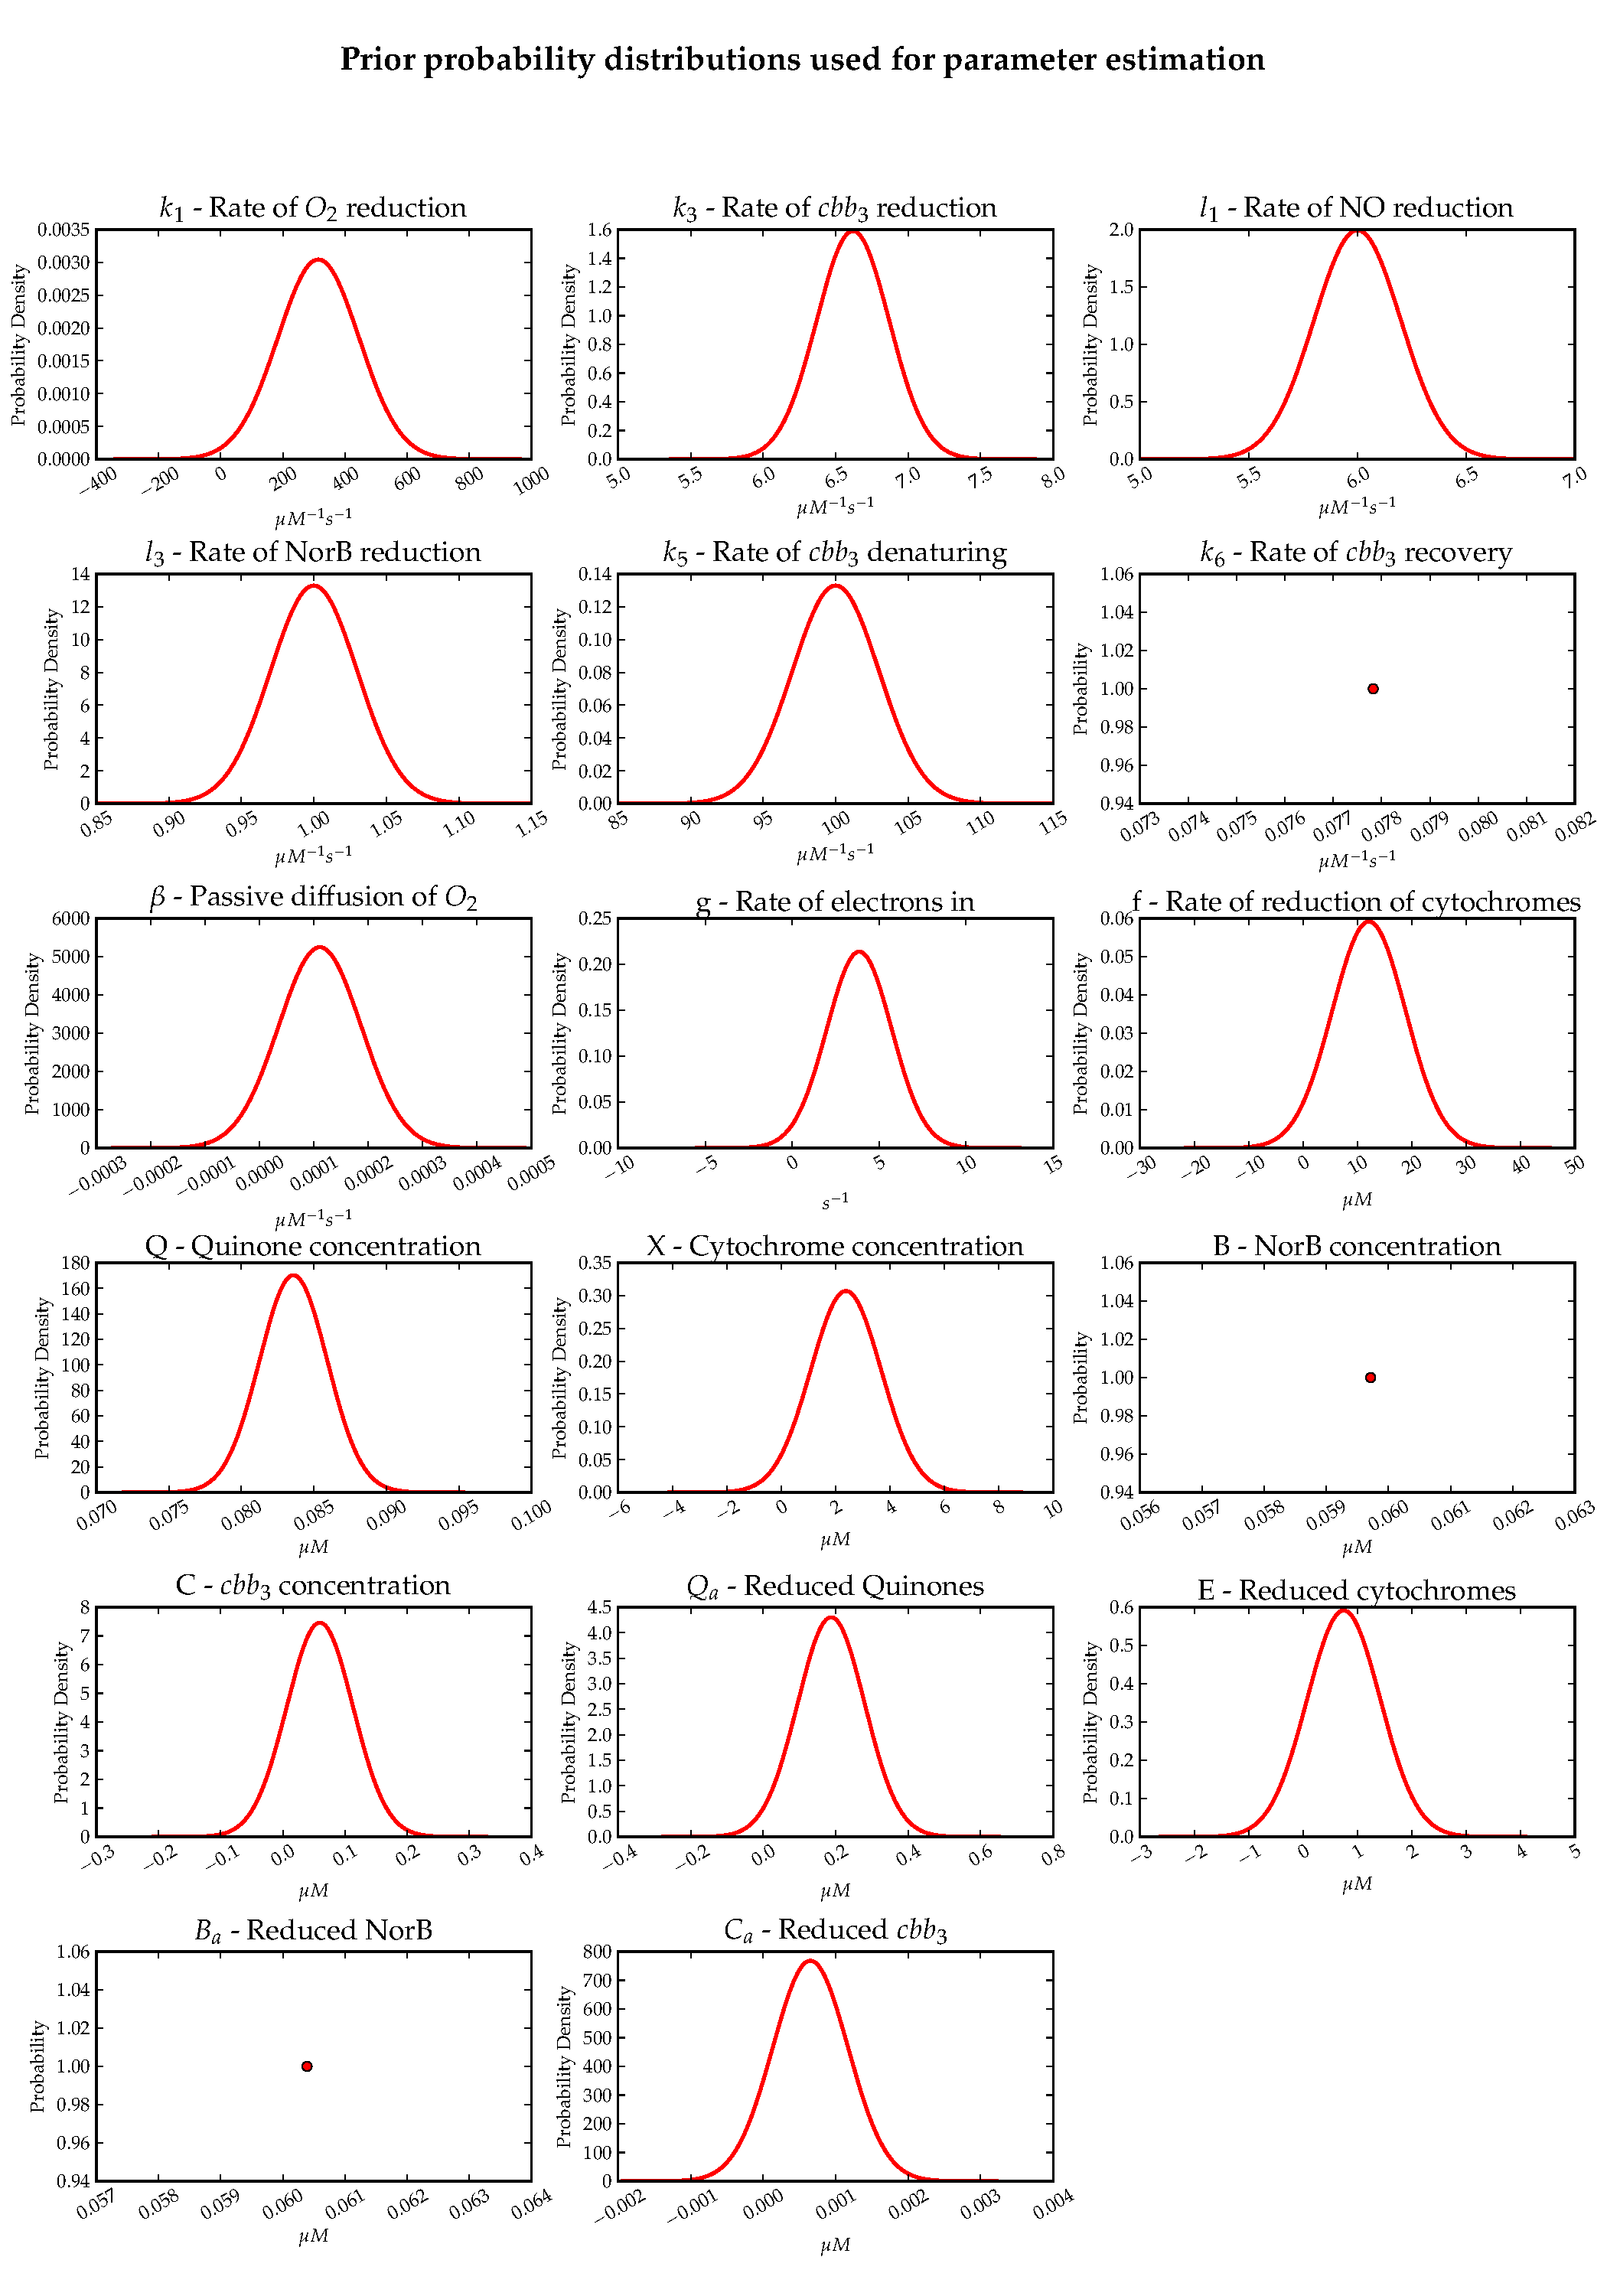
\includegraphics[width=15cm, trim=0cm 0cm 0cm 0cm]{./06-noreduction/data/aer-no-priors.pdf}
 % priors.pdf: 1008x1008 pixel, 72dpi, 35.56x35.56 cm, bb=0 0 1008 1008
 \caption[Prior probability distributions for aerobic nitric oxide reduction]{{\bf Prior probability distributions for aerobic nitric oxide reduction}. These are the probability distributions used as priors by the parameter estimation algorithm.
 \label{fig:aer_no_priors}}
\end{figure}
\afterpage{\clearpage}

\subsubsection{Parameter Estimation Results}
The parameter estimation process was run in the same fashion as that described in Chapter \ref{chap:oxygenreduction}. The 4 experimental datasets were run 20 times (each) for 20,000 iterations using the prior probability distributions shown in Figure \ref{fig:aer_no_priors}. This generated parameter trajectories from each of the 4 datasets. The second dataset (Figure \ref{fig:nodata2}) was still analysed even though it is unlikely that the model will successfully be able to be parametrised from it. Unfortunately upon examination of the \textit{BOF} values from the MHMC output and the best-fitting solved output it was clear that the prior probability distributions in conjunction with the model are incapable of accurately describing the experimental data. This strongly suggested that the new prior probability distributions (those obtained from the literature for the NO related components) were incorrect. The solved output from datasets 3 \& 1 are shown in Figures \ref{fig:nosim1.1} \& \ref{fig:nosim3.1} respectively.

In dataset 3, the reduction of oxygen appears to be being modelled quite accurately. This is due to the largely featureless nature of the reduction curve which can easily be accommodated by the wide prior probability distributions given for the parameters involved. The rate change upon addition of a small amount of nitric oxide is only very slight, thus a perfectly straight line will fit it very well. As can be seen however, nitric oxide removal by diffusion is being modelled very poorly indeed. There is no active NorB in this culture, thus there is no modelled nitric oxide reduction. The prior distribution for the diffusion rate of nitric oxide is clearly incorrect, as nitric oxide removal in the solved output is virtually non-existent.

In dataset 1, reduction of oxygen is being modelled very poorly as the parameters produced by the parameter estimation system do not appear to have captured the behaviour that causes oxygen reduction to cease. In this case the \textit{BOF} value has been minimised by generating a linear reduction of oxygen which doesn't accurately represent either of the observed rates. As has been noted about dataset 3, the rate of nitric oxide diffusion is incorrect, thus in order to obtain a sensible rate for removal/reduction of nitric oxide the rate constants for nitric oxide reduction will have to have been increased artificially. This combination of parameters also means that the reduction in rate of oxygen reduction cannot be modelled correctly. This behaviour should be attributed to temporary chemical inhibition of \cbbthree{} by nitric oxide itself (which is now present in high enough concentrations), and by competition for electrons with NorB.

As in Chapter \ref{chap:oxygenreduction}, the prior probability distributions were incapable of producing parameter sets which accurately model the experimental data, thus making the posterior probability distributions generated invalid. The prior probability distributions were therefore altered in an attempt to improve fitting. In addition to altered prior probability distributions a slightly different parameter estimation protocol was employed which is detailed in the next section.

\begin{figure}[tbp]
 \centering
 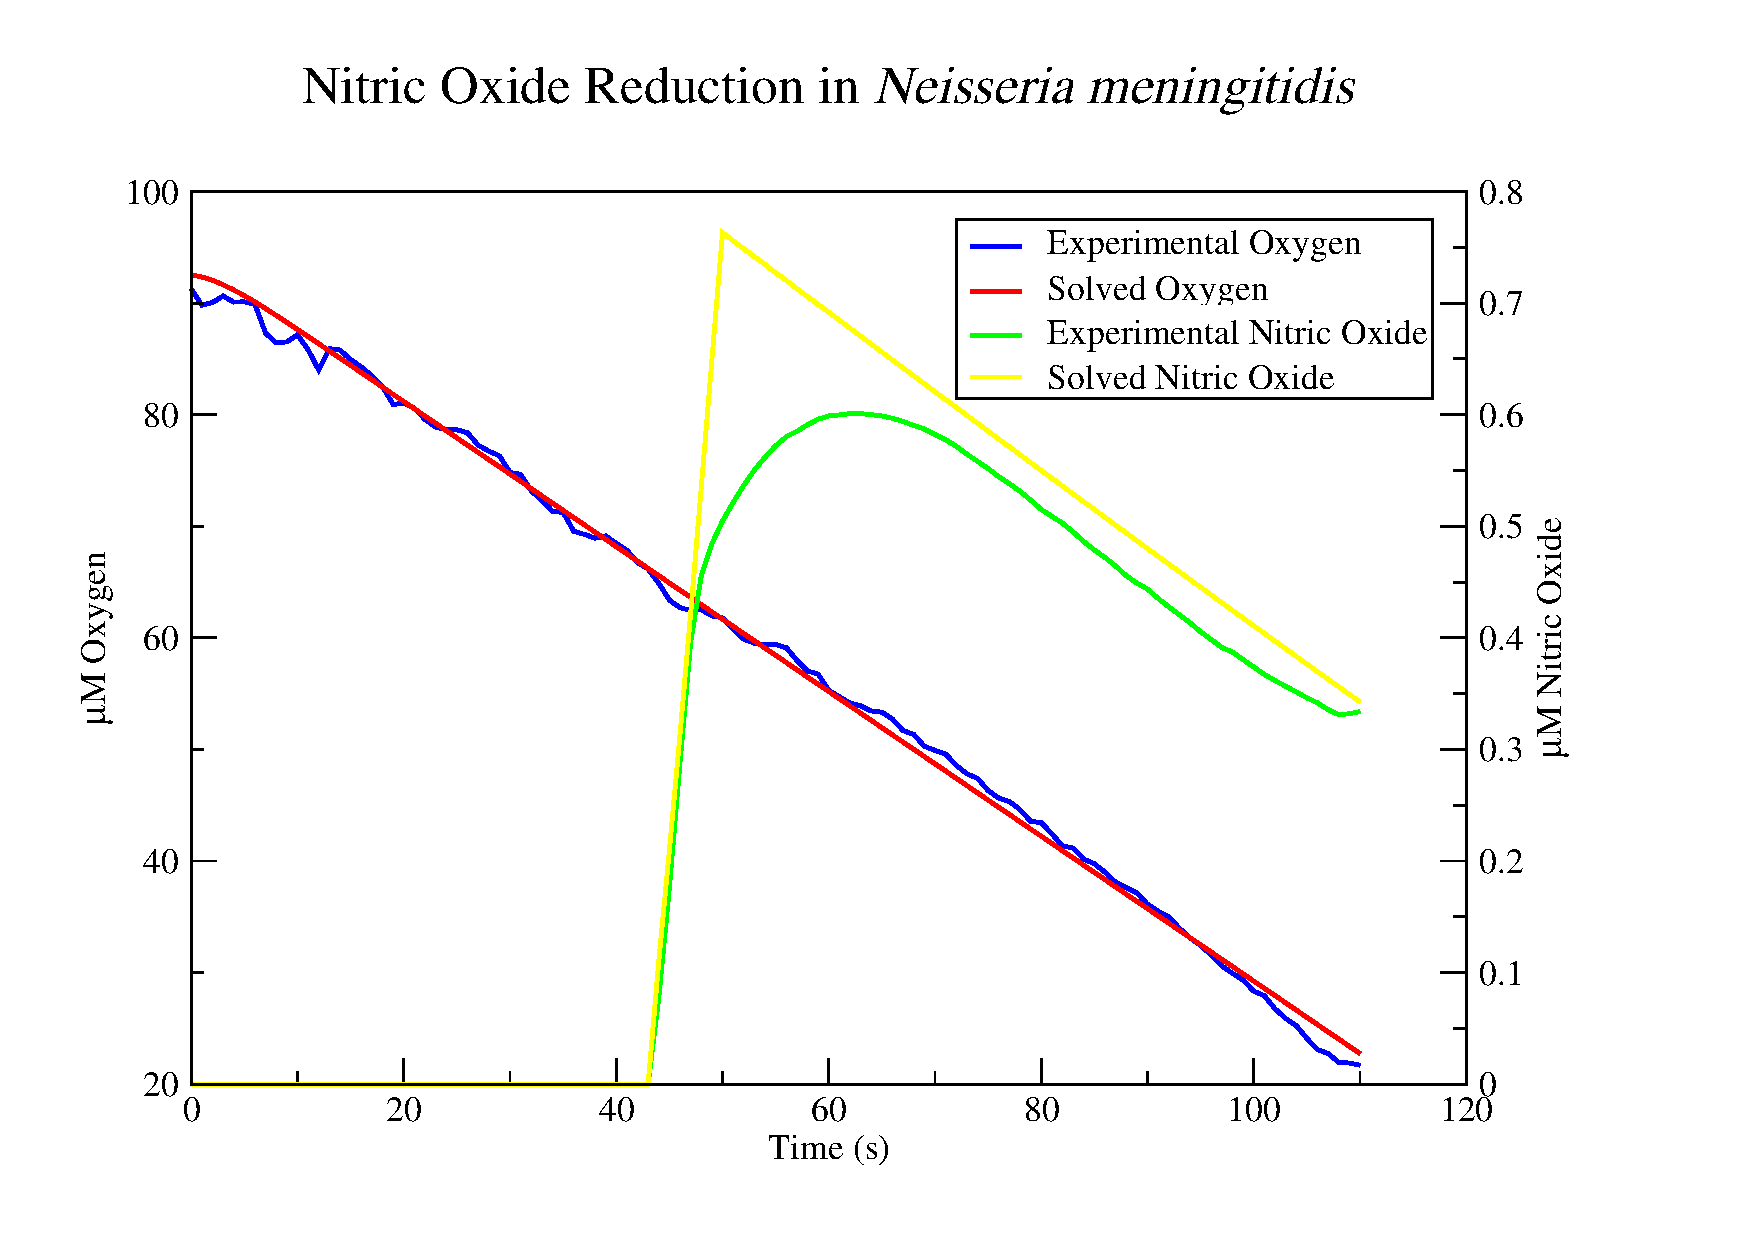
\includegraphics[width=15cm, trim=1cm 1cm 3cm 1cm, clip=true]{./06-noreduction/data/aer-no-sim1.pdf}
 % nosim.eps: 0x0 pixel, 300dpi, 0.00x0.00 cm, bb=0 0 794 595
 \caption[{Nitric Oxide Reduction in \textit{Neisseria meningitidis}.}]{{\bf Nitric Oxide Reduction in \textit{Neisseria meningitidis}.} This figure shows the first attempt at fitting the model to experimental data using priors determined from literature values. Nitric oxide disappearance is not being modelled at all.}
 \label{fig:nosim1.1}
\end{figure}

\begin{figure}[tbp]
 \centering
 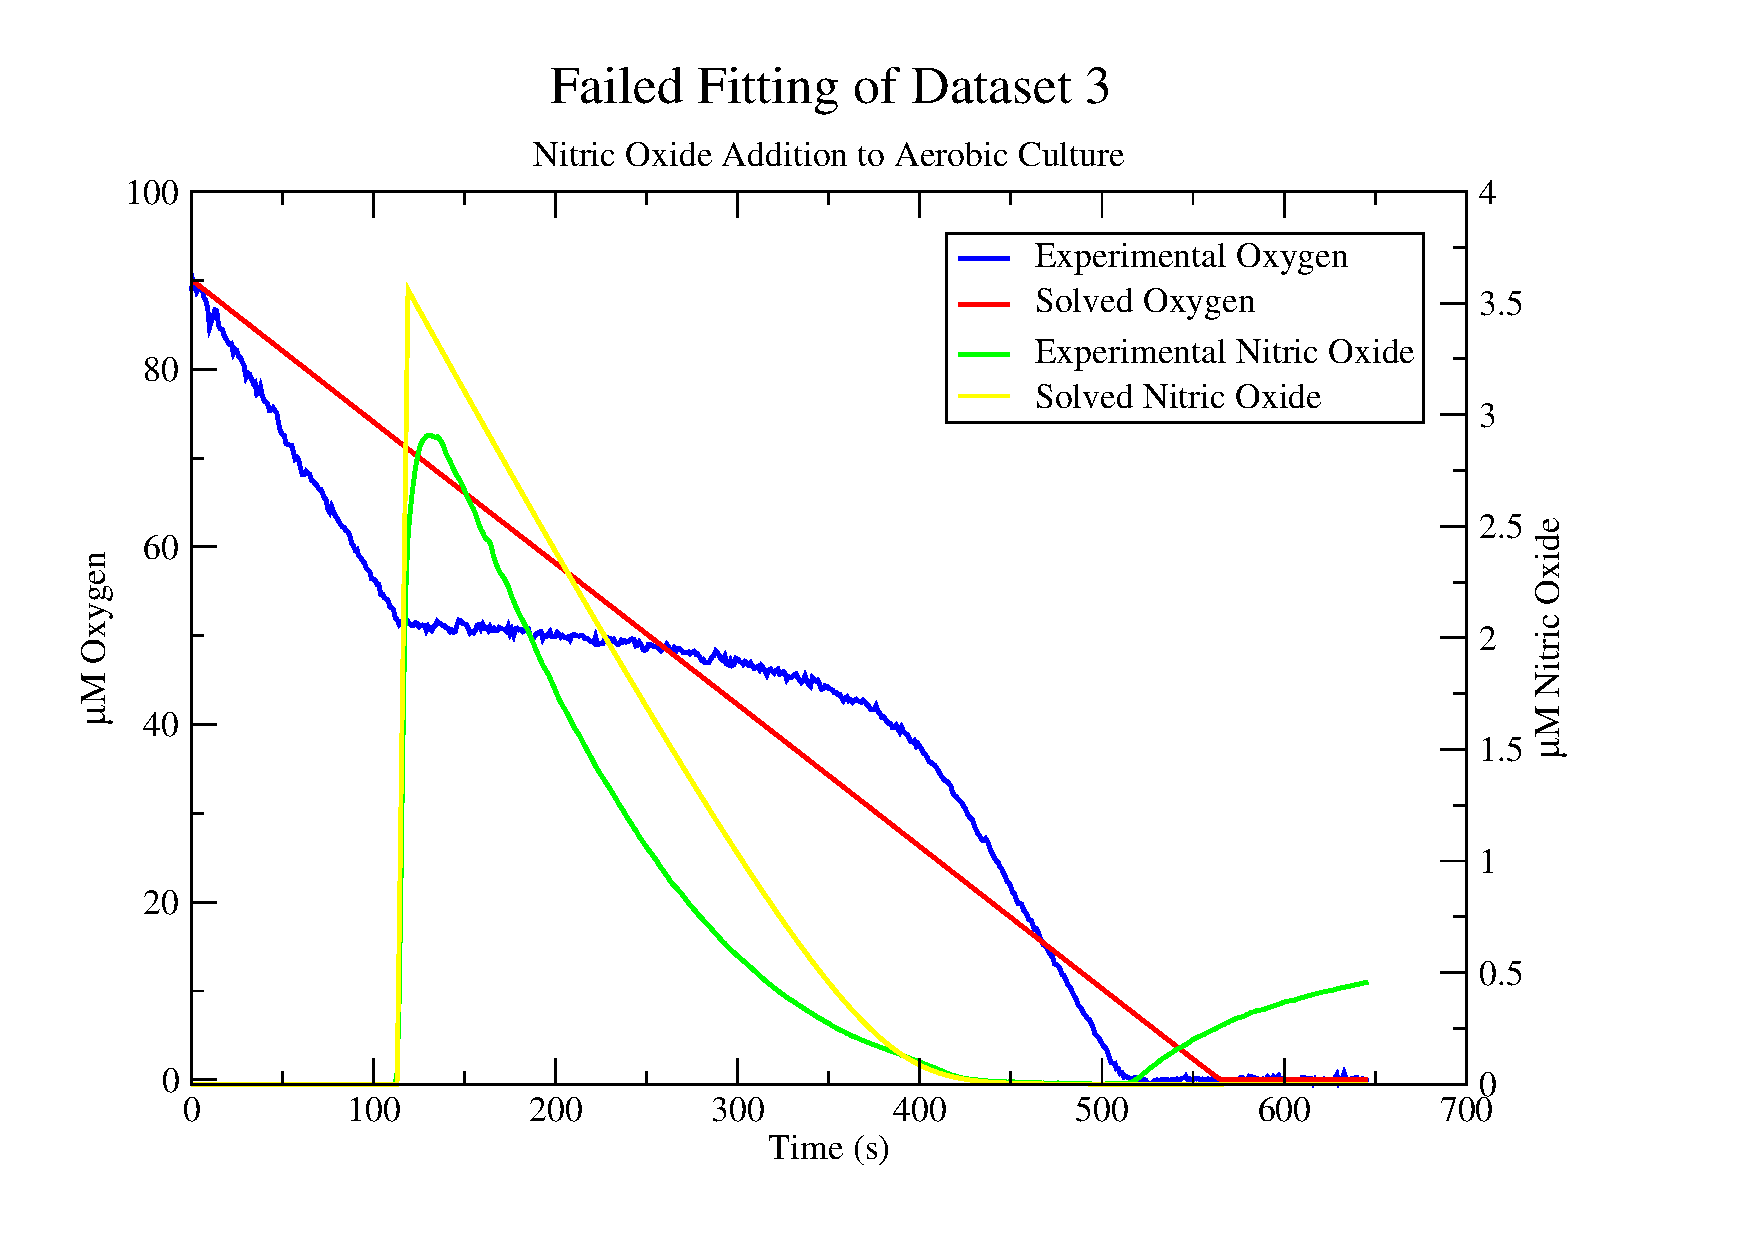
\includegraphics[width=15cm, trim=1cm 1cm 3cm 1cm, clip=true]{./06-noreduction/data/aer-no-sim3.pdf}
 % nosim.eps: 0x0 pixel, 300dpi, 0.00x0.00 cm, bb=0 0 794 595
 \caption[{Nitric Oxide Reduction in \textit{Neisseria meningitidis}.}]{{\bf Nitric Oxide Reduction in \textit{Neisseria meningitidis}.} This figure shows the first attempt at fitting the model to experimental data using priors determined from literature values. Nitric oxide disappearance is now being modelled much more accurately than in Figure \ref{fig:nosim1.1}. Oxygen reduction is not being modelled correctly and the best fitting parameters generate a straight line rather than capturing the stopping and restarting of oxygen reduction.}
 \label{fig:nosim3.1}
\end{figure}

\subsubsection{Adapted Parameter Estimation Protocol}

As dataset 3 was the simplest of the experimental datasets which describe the effects of addition of nitric oxide to aerobically respiring cultures, this dataset could be run as a standalone step in the Bayesian scheme for parameter estimation. This dataset described some of the experimentally observed behaviour in isolation, such as the removal of nitric oxide by diffusion alone, therefore could generate a posterior probability distribution for datasets where that parameter could \textit{not} be examined in isolation. Datasets 1 and 4 ideally required this information as a prior probability distribution as the experimentally observed disappearance of nitric oxide was expected to be due to both diffusion and reduction (by NorB). Therefore dataset 3 could be used to inform the prior probability distribution of datasets 1 and 4. Statistically this did not pose a problem even though the three datasets were run in parallel previously. This was because the numerical output from those previous attempts was not being used as input for the subsequent attempts.

\subsubsection{Secondary Parameter Estimation Results}
Trial and error was employed to produce an initial informed prior value for $\gamma$, the rate of diffusion of nitric oxide, which was the problematic parameter for datasets 3 and 4 previously. This value was estimated to be $\approx 0.02~\mu Ms^{-1}$ based upon visual comparison of the solved output against the experimental data. This value was then used as a prior with no bounds so that the parameter estimation algorithm could home in on the correct distribution. All the other prior probability distributions were left unchanged from the first attempt.

Figure \ref{fig:nosim1.2} shows greatly improved fitting of solved data to experimental values suggesting that the parameters are now correct (or at least reasonably close) for describing the removal of nitric oxide. The model is still not capturing the small effect on oxygen reduction rate visible in the experimental data however. A linear regression of the solved oxygen data suggests that it is in fact a perfectly straight line ($R^2=0.9999$, source data not shown) whereas there should be a slight elbow upon addition of nitric oxide. This was not considered to be a significant problem here, as the effect is far more visible in the subsequent dataset(s), therefore would be more easily modelled.

The posterior probability distribution for $\gamma$ produced by this dataset parameter estimation can be used a prior probability distribution for parameter estimation of datasets 1 and 4, as this now includes the missing information about rate of removal of nitric oxide by diffusion.

\begin{figure}[tbp]
 \centering
 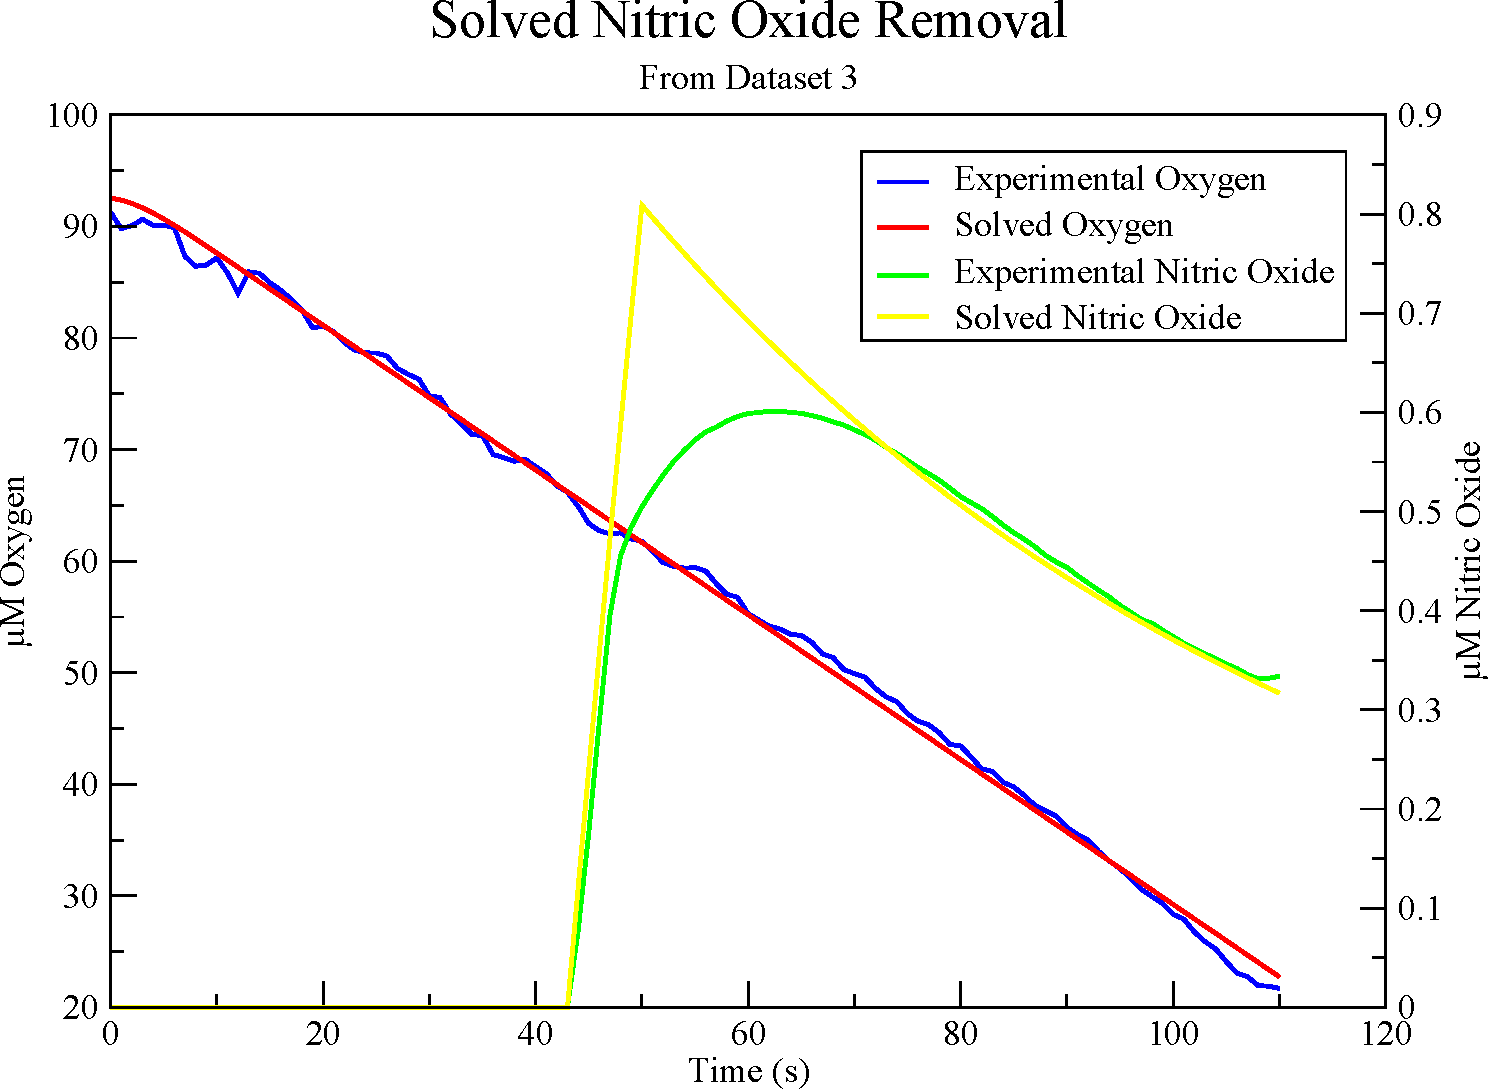
\includegraphics[width=15cm, trim=1cm 1cm 3cm 1cm, clip=true]{./06-noreduction/data/aer-no-sim1-2.pdf}
 % nosim.eps: 0x0 pixel, 300dpi, 0.00x0.00 cm, bb=0 0 794 595
 \caption[{Nitric Oxide Reduction in \textit{Neisseria meningitidis}.}]{{\bf Nitric Oxide Reduction in \textit{Neisseria meningitidis}.} This figure shows the second attempt at fitting the model to experimental data using priors determined from literature values in addition to manually adjusted priors. Oxygen reduction is modelled almost perfectly, and the shape of the nitric oxide reduction curve is captured well also.}
 \label{fig:nosim1.2}
\end{figure}

%no longer include this as it is wrong
%\begin{figure}[p]
% \centering
% 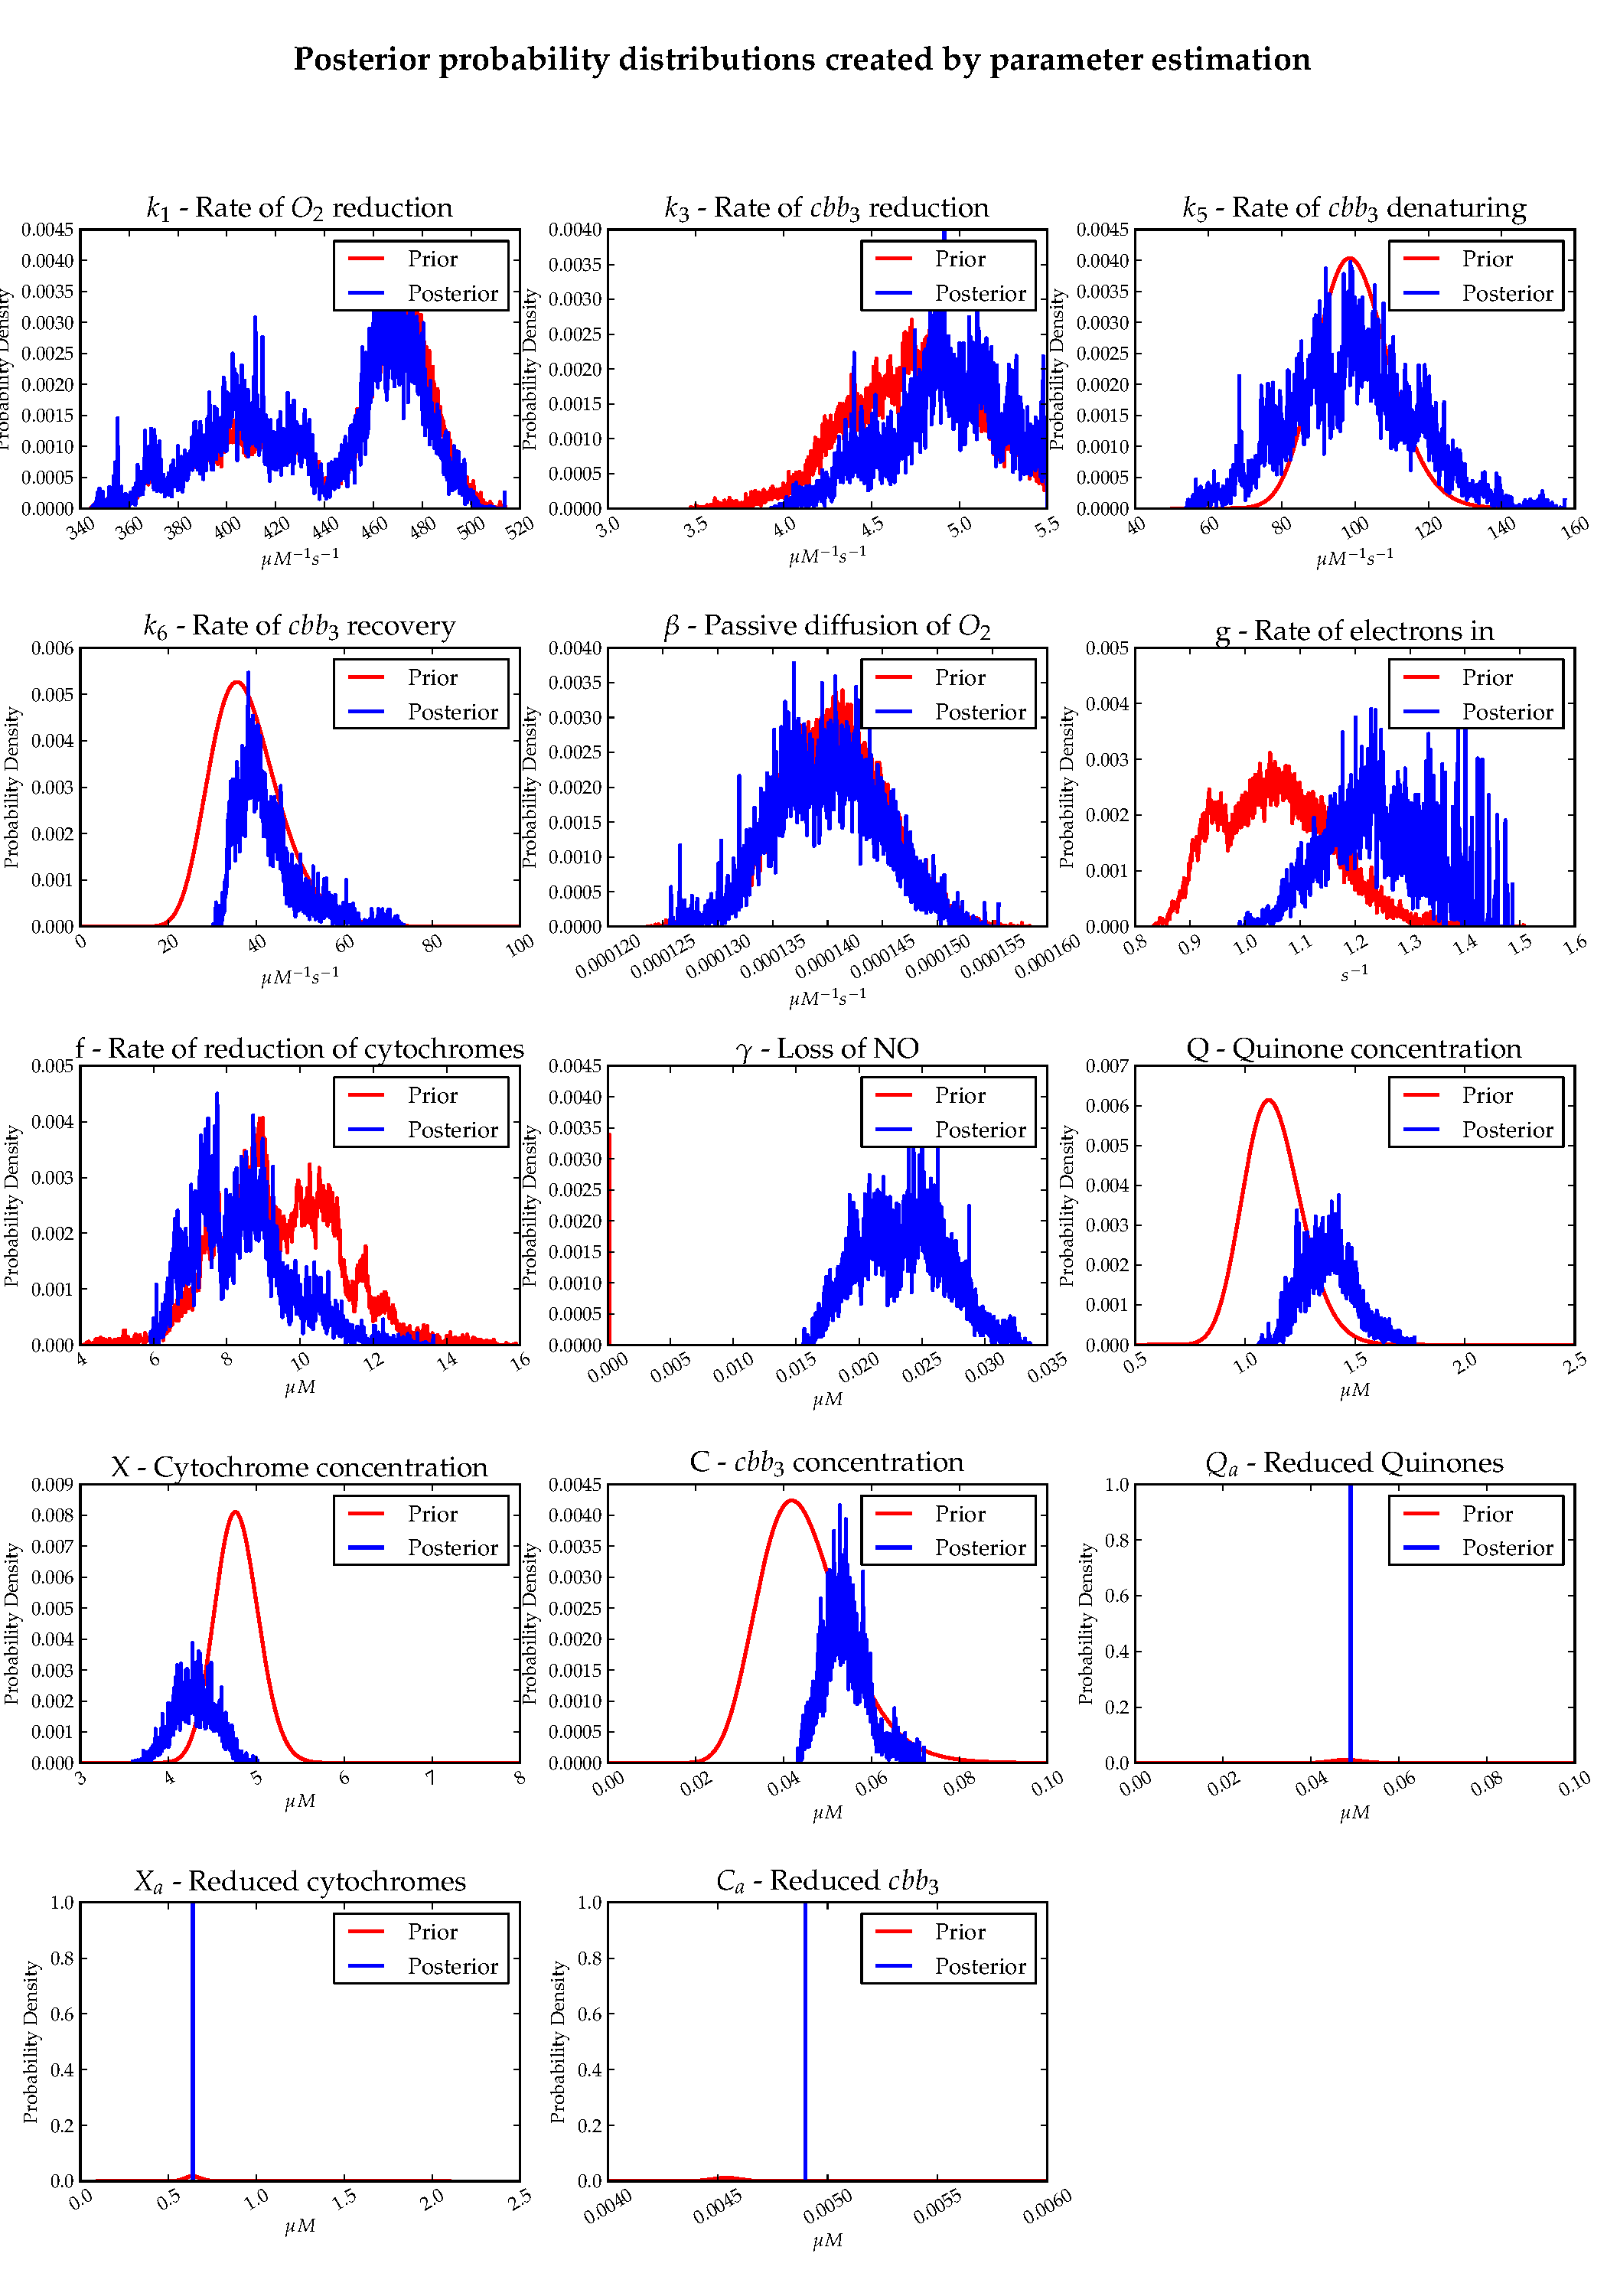
\includegraphics[width=15cm, trim=0cm 0cm 0cm 0cm]{./06-noreduction/data/posteriors-1.pdf}
% % priors.pdf: 1008x1008 pixel, 72dpi, 35.56x35.56 cm, bb=0 0 1008 1008
% \caption[Posterior Distributions for Dataset 1]{{\bf Posterior Distributions for Dataset 1}. The posterior probability distributions for dataset 1 of nitric oxide removal. All the parameters are still well within their prior bounds with the exception of $\gamma$ which had a manually altered starting value which was significantly different from the original prior distribution. The initial reduced state posteriors appear as point values as the perturbation kernel was disabled for these values (starting value is largely irrelevant).
% \label{fig:dataset1posterior1}}
%\end{figure}

\subsubsection{Tertiary Parameter Estimation Results}
The third round of parameter estimation built upon the results from the previous section. After parametrising the value for $\gamma$ from dataset 3, it was then possible to attempt parameter estimation on datasets 1 and 4 which also involved $l_1$, $l_3$, $k_5$ \& $k_6$ for reduction of nitric oxide and inactivation of \cbbthree{} by nitric oxide respectively. The prior probability distributions used for this round of parameter estimation were the same as in Figure \ref{fig:aer_no_priors} except that the distribution for $\gamma$ was replaced by that found in the previous section.

Preliminary test runs (data not shown) using these prior probability distributions suggested that at least one of the two parameters relating to the inactivation of \cbbthree{} by nitric oxide was incorrect for this model. In order to obtain a oxygen reduction curve that matches the general shape of the experimentally obtained data a ratio of $k_5:k_6 \approx 2000:1$ was required. Since it was unknown which of the two values was more incorrect, both parameters were allowed to be perturbed freely during parameter estimation, i.e. they had no prior probability distribution. Unfortunately this seemed to be the only sensible approach to take given the lack of further data. These preliminary runs suggested that the number of parameter estimation iterations would need to be increased for this dataset also due to the presence of local \textit{BOF} value minima caused by the model fitting oxygen as a straight line between the fixed starting point and the point at which oxygen is depleted similar to the result shown in Figure \ref{fig:nosim3.1}. Figure \ref{fig:nosim3-bof} illustrates local minima phenomenon. Given that this figure shows that a suitably low \textit{BOF} value is not achieved until at least 15000 iterations (and in some cases this extended up to 50000 iterations) a value of 100000 iterations was chosen to ensure that a significant number of data-points were available to generate posterior probability distributions.

\begin{figure}[tbp]
 \centering
 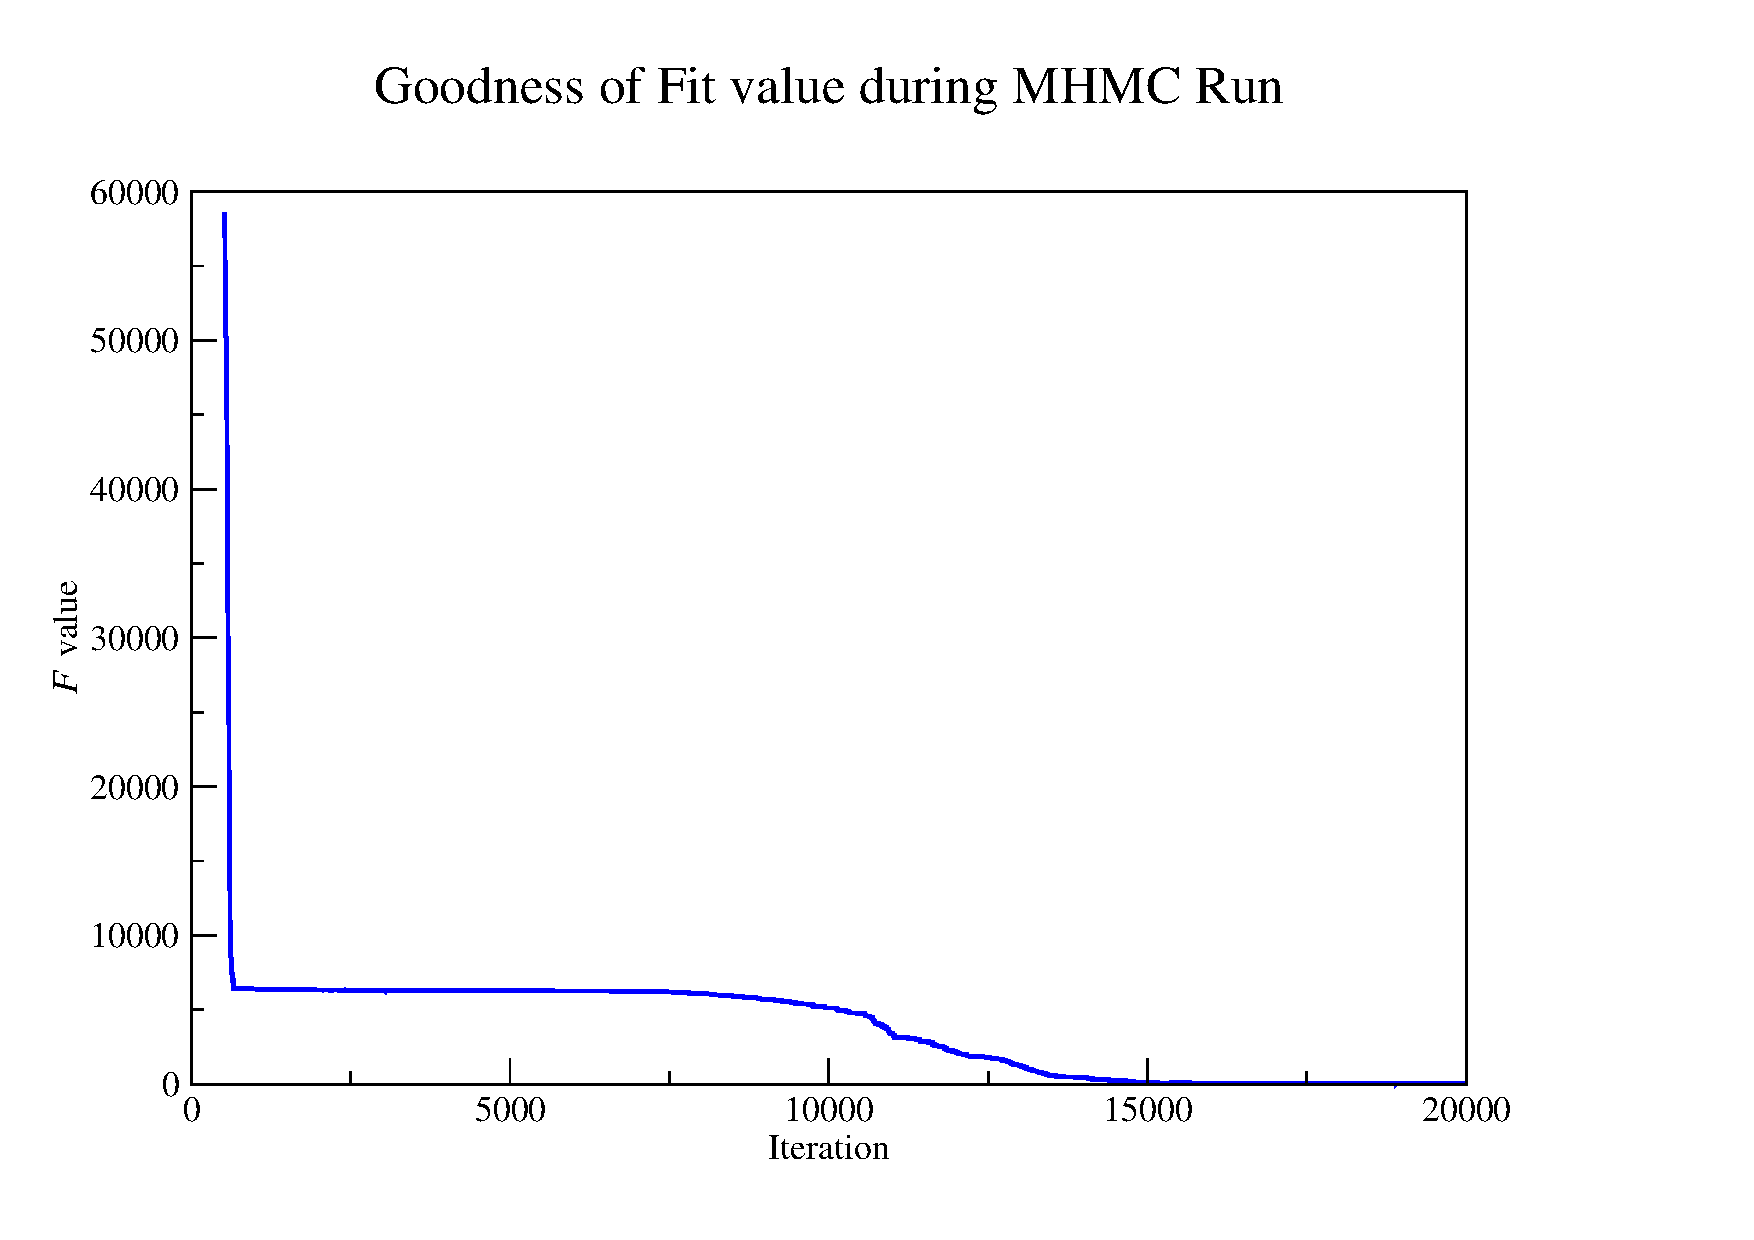
\includegraphics[width=15cm, trim=0.5cm 1cm 3cm 1cm, clip=true]{./06-noreduction/data/ds3-bof.pdf}
 % nosim.eps: 0x0 pixel, 300dpi, 0.00x0.00 cm, bb=0 0 794 595
 \caption[{Local Fitness Minima During Parameter Estimation.}]{{\bf Local Fitness Minima During Parameter Estimation.} This figure shows the \textit{BOF} value as the MHMC progresses on dataset 1. A local fitness minima is clearly visible at a \textit{BOF} value of approximately 7000 where the parameter estimation algorithm has settled on a straight line for oxygen reduction. After a variable number of iterations the MHMC run exits the local fitness minima and progresses towards a much better fitting set of parameters. This is a typical plot of the \textit{BOF} values, however in some runs the fitness minima is exited much more abruptly rather than the gradual change seen here.}
 \label{fig:nosim3-bof}
\end{figure}

A representative plot showing the solved data after running the parameter estimation system as described above is shown in Figure \ref{fig:nosim3.2}. The model appeared to be able to capture all the features of the oxygen reduction curve including the halting of oxygen reduction upon addition of nitric oxide, and the recovery after nitric oxide has been removed. Similarly to the results seen in Chapter \ref{chap:oxygenreduction} the high degree of \cbbthree{} for oxygen is also captured (probably a little too high). Nitric oxide was generally modelled less well than was hoped. The point of nitric oxide depletion appeared to be modelled correctly, but the rate of reduction of nitric oxide starts too fast and slows too quickly resulting in more pronounced curvature than the experimental data shows.

The concentration of nitric oxide present will also affect the rate of \cbbthree{} reduction (due to the effect of temporary inactivation by nitric oxide), thus implying that the rate constants obtained to describe that effect may not be completely correct. Some of the observed discrepancy between the experimental and solved nitric oxide concentrations may in fact be due to errors introduced into the experimental data by the experimental set up. The nitric oxide electrode was not capable of detecting large changes in concentration quickly and this always resulted in a lag between nitric oxide addition and detection by the electrode. This is obvious in the experimental datasets where the total nitric oxide addition is not captured as the cultures have already started to remove it. This requires backwards extrapolation of the experimental data to determine what the actual added concentration was (and what should be added \textit{in silico} to the model).

\begin{figure}[tbp]
 \centering
 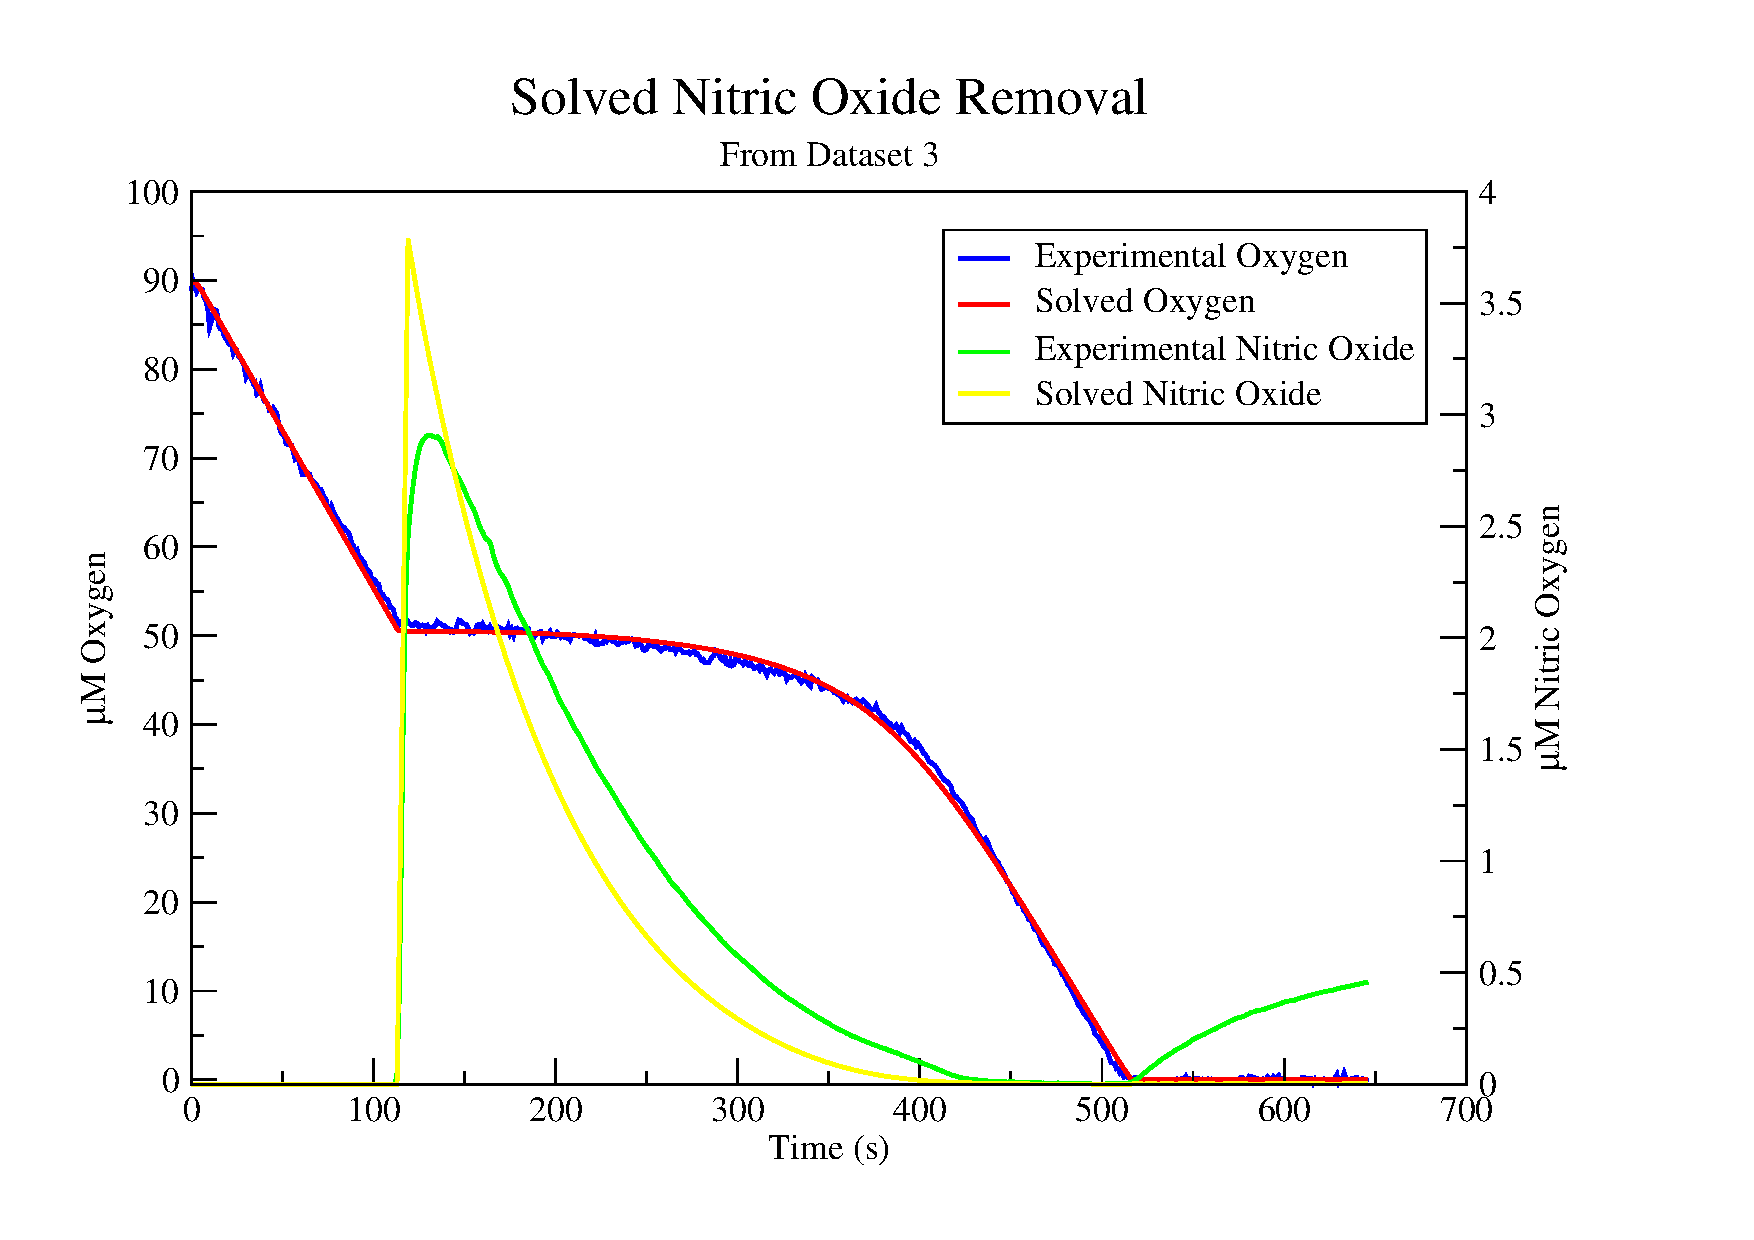
\includegraphics[width=15cm, trim=1cm 1cm 3cm 1cm, clip=true]{./06-noreduction/data/aer-no-sim3-1.pdf}
 % nosim.eps: 0x0 pixel, 300dpi, 0.00x0.00 cm, bb=0 0 794 595
 \caption[{Nitric Oxide Reduction in \textit{Neisseria meningitidis}.}]{{\bf Nitric Oxide Reduction in \textit{Neisseria meningitidis}.} This figure shows the third attempt at fitting the model to experimental data using priors determined from literature values in addition to manually adjusted priors. Oxygen reduction is being modelled remarkably well, whereas the rate of nitric oxide reduction appears to be slightly too high in the solved output.}
 \label{fig:nosim3.2}
\end{figure}

The posterior probability distributions generated from this third round of parameter estimation are shown in Figure \ref{fig:redoneposterior2}. The distributions generated for the parameters relating solely to oxygen reduction were broadly similar to the prior probability distributions which was to be expected and confirms that these distributions capable of describing the oxygen reduction behaviour. The rate of NO reduction by NorB appeared to be very similar to the prior probability distribution however the rate of NorB reduction seemed to have been vastly overestimated in the prior distribution. The prior distribution for this parameter was unknown however, and was set to a very wide lognormal with mean of 1. The rate of NO diffusion ($\gamma$) tended to settle at the lower end of the prior distribution. The most interesting posterior probability distributions were those of $k_5$ and $k_6$ which actually had to be freely perturbed, rather than be constrained by their prior probability distributions. Neither of these two parameters settled anywhere near the prior probability distributions. $k_5$ never settles on a value less than $\approx 400~\mu M^{-1}s^{-1}$. This value turned out to be a critical threshold to at which the inactivation of \cbbthree{} occurs. At lower values of $k_5$ the inactivation is slower than observed in the experimental dataset and the in the solved data the ``elbow'' is shifted visibly to the right. At or above this threshold the inactivation point closely matches that seen in the experimental dataset. It appeared that that absolute values of $k_5$ and $k_6$ are unimportant, only that $k_5$ is greater than $\approx 400~\mu M^{-1}s^{-1}$ and that the ratio of $k_5:k_6 \approx 2000:1$. Unfortunately this meant that it was impossible to determine if the obtained posterior probability distributions were actually representative of the true distributions.

\begin{figure}[p]
 \centering
 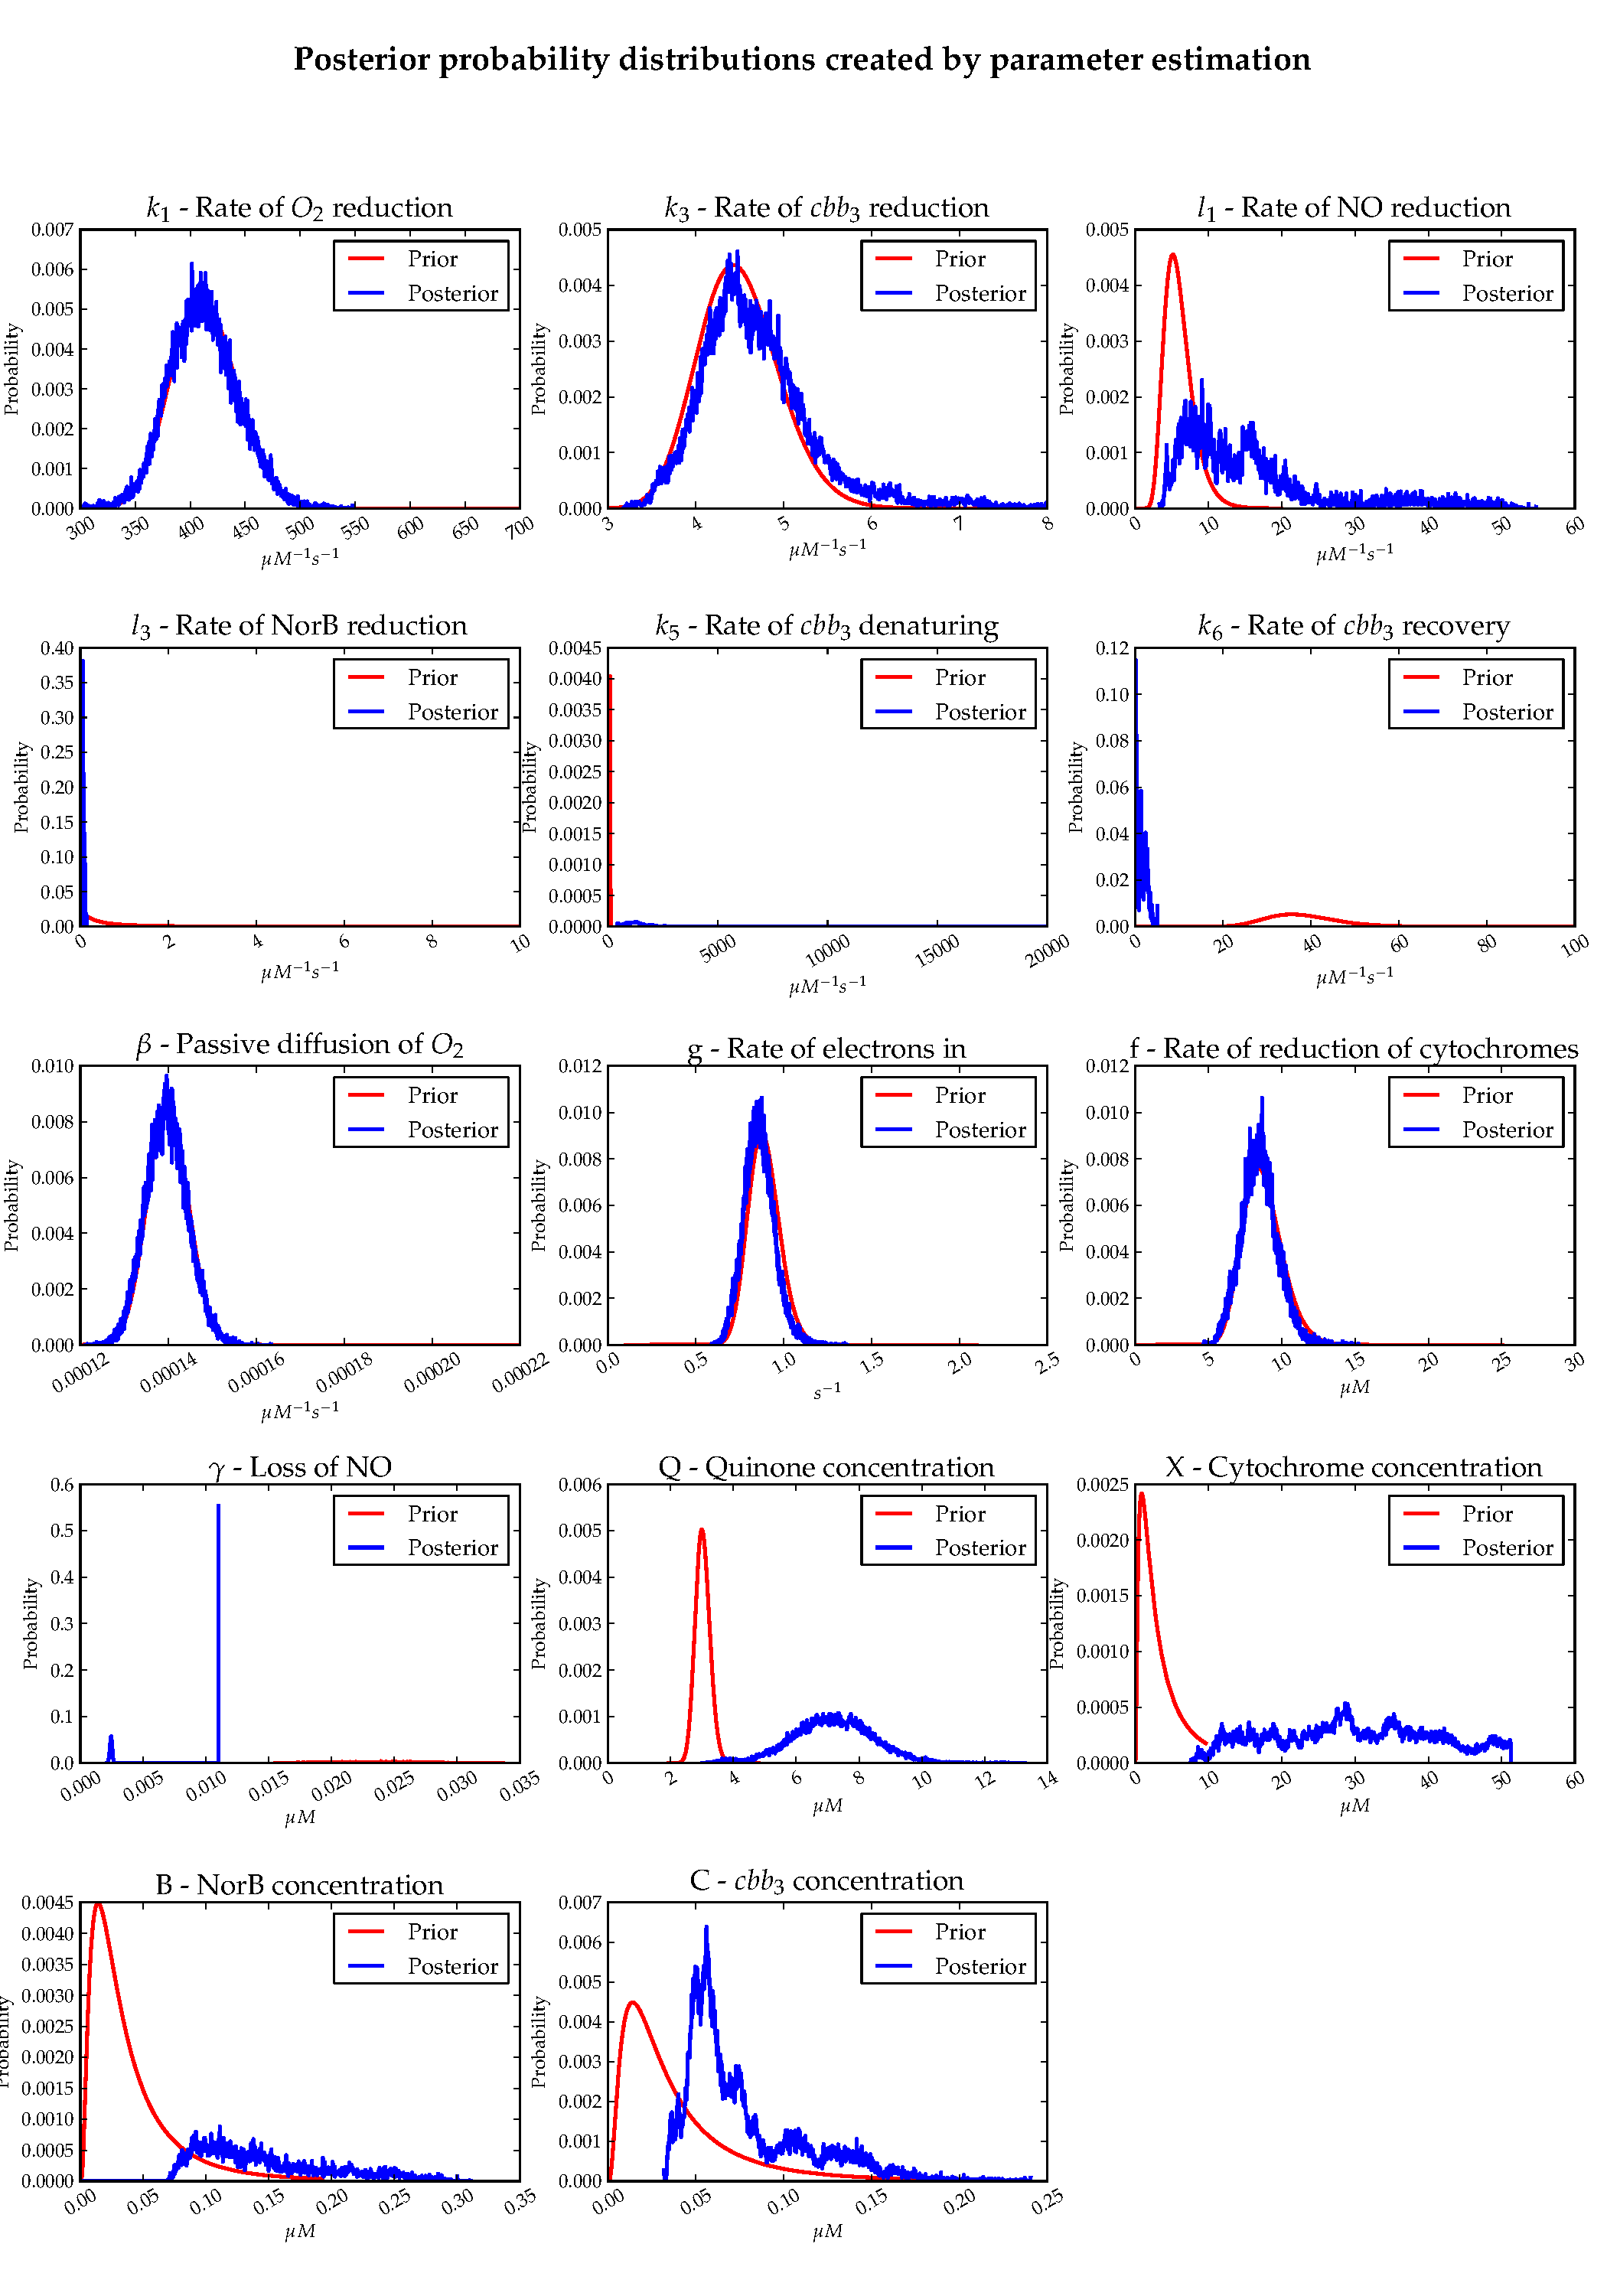
\includegraphics[width=15cm, trim=0cm 0cm 0cm 0cm]{./06-noreduction/data/posteriors-redo2.pdf}
 % priors.pdf: 1008x1008 pixel, 72dpi, 35.56x35.56 cm, bb=0 0 1008 1008
 \caption[Posterior Distributions for Datasets 1 and 4]{{\bf Posterior Distributions for Datasets 1 and 4}. The posterior probability distributions for datasets 1 and 4 of nitric oxide removal.
 \label{fig:redoneposterior2}}
\end{figure}
A comparison between the prior and posterior distributions can be seen in tabular form in Table \ref{tab:redone-prob-stat}. This table shows the parameters of the idealised lognormal distributions which describe the obtained probability distributions to more easily represent the data.

\begin{table}[tbp]%needs to be 'here' as section is short
\renewcommand{\arraystretch}{1.5}
\begin{center}
\begin{tabular}{cccccc}
\toprule
& & \multicolumn{2}{c}{\textbf{Priors}} & \multicolumn{2}{c}{\textbf{Posteriors}} \\
\textbf{Parameter} && ${\bar{x}}$ & $\sigma$ & ${\bar{x}}$ & $\sigma$\\
\midrule
$k_1$ && 413.228 & 30.046 & 417.88 & 31.172\\
$k_3$ && 4.496 & 0.463 & 4.65 & 0.619\\
$l_1$ && 6 & 2 & 13.12$\uparrow$ & 8.321$\uparrow$\\
$l_3$ && 1 & 2 & 0.058$\downarrow$ & 0.021$\downarrow$\\
$k_5$ && 100 & 10 & 1741.8$\uparrow$ & 1822.0$\uparrow$\\
$k_6$ && 38 & 8 & 1.076$\downarrow$ & 1.473$\downarrow$\\
$\beta$ && 0.00014 & $4.72\times 10^{-6}$ & 0.00014 & $4.7\times 10^{-6}$\\
g && 0.889 & 0.089 & 0.857 & 0.086\\
f && 8.707 & 1.35 & 8.398 & 1.237\\
$\gamma$ && 0.017 & 0.0015 & \\
Q && 3.143 & 0.240 & 7.06 & 1.317\\
X && 4.732 & 6.707 & 27.45 & 12.08\\
B && 0.043 & 0.044 & 0.137 & 0.048\\
C && 0.043 & 0.044 & 0.071 & 0.029\\
\bottomrule
\end{tabular}
\end{center}
\caption[Posterior Probability Statistics]{{\bf Posterior Probability Statistics.} This table shows the parameters required to create lognormal distributions that describe the prior and posterior probability distributions. The values for the priors are as in Table \ref{tab:noProbstat1}. The posterior distributions were generated from dataset 3 (after being run on dataset 1), and where they relate to concentrations, these have been normalised. The lognormal distributions represent best-fits to the actual posterior distributions. Where there are significant differences between the prior and posterior values for either the mean or standard deviation, these are indicated by $\uparrow$ and $\downarrow$.
\label{tab:redone-prob-stat}}
\end{table}
\subsubsection{Analysis of Convergence}
The Gelman-Rubin R statistics were calculated for the Monte-Carlo trajectories for each parameter and these are presented in Table \ref{tab:noRstat-redone}. The newly included parameters all had large R statistic values suggesting that there is still opportunity for scale reduction in the trajectories. This is highly likely to be due to the fact that $k_5$ and $k_6$ had to be unconstrained by prior probability distributions, and they are directly affecting the values of $l_1$ and $l_3$ in such a way as to prevent them converging fully. This is especially true of $l_3$ which has an extremely high R statistic. This actually suggests that $l_3$ is a long way away from being fully converged, or that an anomalous Markov Chain has been included.

\begin{table}[tbp]%needs to be 'here' as section is short
\renewcommand{\arraystretch}{1.5}
\begin{center}
\begin{tabular}{ccc|ccc}
\toprule
\textbf{Parameter} && \textbf{R Statistic} & \textbf{Parameter} && \textbf{R Statistic}\\
\midrule
$k_1$ && 1.15 & g && 1.13\\
$k_3$ && 1.31 & f && 1.20\\
$l_1$ && 4.92 & $\gamma$ && \\
$l_3$ && 131.447 & Q && 1.54\\
$k_5$ && 6.46 & X && 3.82\\
$k_6$ && 7.37 & B && 6.74\\
$\beta$ && 1.02 & C && 2.92 \\
\bottomrule
\end{tabular}
\end{center}
\caption[Gelman-Rubin Convergence Statistic]{{\bf Gelman-Rubin Convergence Statistic.} This table shows the Gelman-Rubin Convergence statistic for all the Markov chains from dataset 3. For parameters which are concentrations, the statistic relates to the values after normalisation (data is normalised based on initial oxygen reduction rate).
\label{tab:noRstat-redone}}
\end{table}

\subsubsection{Analysis of Correlation}
A correlation analysis was performed on each of the parameters using the Monte-Carlo trajectories as in Chapter \ref{chap:oxygenreduction}. The upper-triangle correlation matrices are shown in Tables \ref{tab:noregress1} and \ref{tab:noregress4}. There was a very strong positive correlation between $k_5$ and $k_6$, which given the brief discussion earlier in the chapter was to be expected. As it appeared that the ratio and not the absolute values of $k_5$ and $k_6$ was important, a strong positive correlation between values would achieve this.
\begin{table}[p]
\setlength{\tabcolsep}{5pt}
\renewcommand{\arraystretch}{1.5}
  \centering
  \rotatebox{90}{
  \begin{minipage}{24.4cm}
  \centering
  \begin{tabular}{|c|c|c|c|c|c|c|c|c|c|c|c|c|}
    \hline
    \cellcolor{dark-gray} & \cellcolor{dark-gray}$k_1$ & \cellcolor{dark-gray}$k_3$ & \cellcolor{dark-gray}$l_1$ & \cellcolor{dark-gray}$l_3$ & \cellcolor{dark-gray}$k_5$ & \cellcolor{dark-gray}$k_6$ & \cellcolor{dark-gray}g & \cellcolor{dark-gray}f & \cellcolor{dark-gray}Q & \cellcolor{dark-gray}X & \cellcolor{dark-gray}B & \cellcolor{dark-gray}C \\
    \hline
    \cellcolor{dark-gray}$k_1$ & \cellcolor{light-gray}1 & -0.22 & 0.07 & -0.06 & 0.07 & -0.04 & -0.01 & -0.06 & -0.01 & 0.04 & 0.02 & 0 \\
    \hline
    \cellcolor{dark-gray}$k_3$ & \cellcolor{light-gray} & \cellcolor{light-gray}1 & -0.28 & 0.12 & 0.25 & 0.22 & 0.05 & 0.22 & 0.63 & -0.29 & -0.01 & -0.01 \\
    \hline
    \cellcolor{dark-gray}$l_1$ & \cellcolor{light-gray} & \cellcolor{light-gray} & \cellcolor{light-gray}1 & 0.12 & \cellcolor{orange}-0.45 & \cellcolor{orange}-0.52 & -0.09 & 0.06 & -0.20 & -0.25 & -0.11 & \cellcolor{orange}0.32 \\
    \hline
    \cellcolor{dark-gray}$l_3$ & \cellcolor{light-gray} & \cellcolor{light-gray} & \cellcolor{light-gray} & \cellcolor{light-gray}1 & \cellcolor{orange}-0.43 & \cellcolor{orange}-0.40 & -0.083 & 0.16 & -0.07 & -0.15 & \cellcolor{green}-0.81 & 0.04 \\
    \hline
    \cellcolor{dark-gray}$k_5$ & \cellcolor{light-gray} & \cellcolor{light-gray} & \cellcolor{light-gray} & \cellcolor{light-gray} & \cellcolor{light-gray}1 & \cellcolor{green}0.76 & 0.04 & -0.15 & -0.10 & -0.11 & \cellcolor{orange}0.46 & 0.08 \\
    \hline
    \cellcolor{dark-gray}$k_6$ & \cellcolor{light-gray} & \cellcolor{light-gray} & \cellcolor{light-gray} & \cellcolor{light-gray} & \cellcolor{light-gray} & \cellcolor{light-gray}1 & 0.25 & -0.06 & -0.02 & \cellcolor{orange}0.45 & \cellcolor{orange}0.34 & \cellcolor{orange}-0.48 \\
    \hline
    \cellcolor{dark-gray}g & \cellcolor{light-gray} & \cellcolor{light-gray} & \cellcolor{light-gray} & \cellcolor{light-gray} & \cellcolor{light-gray} & \cellcolor{light-gray} & \cellcolor{light-gray}1 & 0.02 & 0 & 0.27 & 0.02 & -0.22 \\
    \hline
    \cellcolor{dark-gray}f & \cellcolor{light-gray} & \cellcolor{light-gray} & \cellcolor{light-gray} & \cellcolor{light-gray} & \cellcolor{light-gray} & \cellcolor{light-gray} & \cellcolor{light-gray} & \cellcolor{light-gray}1 & -0.06 & -0.20 & -0.10 & 0.14 \\
    \hline
    \cellcolor{dark-gray}Q & \cellcolor{light-gray} & \cellcolor{light-gray} & \cellcolor{light-gray} & \cellcolor{light-gray} & \cellcolor{light-gray} & \cellcolor{light-gray} & \cellcolor{light-gray} & \cellcolor{light-gray} & \cellcolor{light-gray}1 & 0.18 & \cellcolor{orange}-0.39 & -0.19\\
    \hline
    \cellcolor{dark-gray}X & \cellcolor{light-gray} & \cellcolor{light-gray} & \cellcolor{light-gray} & \cellcolor{light-gray} & \cellcolor{light-gray} & \cellcolor{light-gray} & \cellcolor{light-gray} & \cellcolor{light-gray} & \cellcolor{light-gray} & \cellcolor{light-gray}1 & -0.05 & \cellcolor{green}-0.87 \\
    \hline
    \cellcolor{dark-gray}B & \cellcolor{light-gray} & \cellcolor{light-gray} & \cellcolor{light-gray} & \cellcolor{light-gray} & \cellcolor{light-gray} & \cellcolor{light-gray} & \cellcolor{light-gray} & \cellcolor{light-gray} & \cellcolor{light-gray} & \cellcolor{light-gray} & \cellcolor{light-gray}1 & 0.11 \\
    \hline
    \cellcolor{dark-gray}C & \cellcolor{light-gray} & \cellcolor{light-gray} & \cellcolor{light-gray} & \cellcolor{light-gray} & \cellcolor{light-gray} & \cellcolor{light-gray} & \cellcolor{light-gray} & \cellcolor{light-gray} & \cellcolor{light-gray} & \cellcolor{light-gray} & \cellcolor{light-gray} & \cellcolor{light-gray}1 \\
    \hline
  \end{tabular}
  \caption[Regression Analysis of Nitric Oxide Reduction Parameters]{{\bf Regression Analysis of Nitric Oxide Reduction Parameters for Dataset 1.} This table shows the $r$ values from linear regression analysis on the parameter trajectories for nitric oxide reduction. Parameters with high correlation have been coloured green ($R\geq0.8$) and those with moderation correlation have been coloured orange ($0.8>R\geq0.3$).
  \label{tab:noregress1}}
  \end{minipage}
  }
\end{table}
\afterpage{\clearpage}

\begin{table}[p]
\setlength{\tabcolsep}{5pt}
\renewcommand{\arraystretch}{1.5}
  \centering
  \rotatebox{90}{
  \begin{minipage}{24.4cm}
  \centering
  \begin{tabular}{|c|c|c|c|c|c|c|c|c|c|c|}
    \hline
    \cellcolor{dark-gray} & \cellcolor{dark-gray}$k_1$ & \cellcolor{dark-gray}$k_3$ & \cellcolor{dark-gray}$k_5$ & \cellcolor{dark-gray}$k_6$ & \cellcolor{dark-gray}g & \cellcolor{dark-gray}f & \cellcolor{dark-gray}Q & \cellcolor{dark-gray}X & \cellcolor{dark-gray}B & \cellcolor{dark-gray}C \\
    \hline
    \cellcolor{dark-gray}$k_1$ & \cellcolor{light-gray}1 & -0.14 & -0.02 & -0.25 & 0.02 & 0.03 & 0.07 & 0.13 & 0.02 & 0.04 \\
    \hline
    \cellcolor{dark-gray}$k_3$ & \cellcolor{light-gray} & \cellcolor{light-gray}1 & 0.05 & 0.21 & -0.08 & -0.02 & -0.08 & -0.29 & \cellcolor{orange}-0.31 & -0.18 \\
    \hline
    \cellcolor{dark-gray}$k_5$ & \cellcolor{light-gray} & \cellcolor{light-gray} & \cellcolor{light-gray}1 & \cellcolor{green}0.74 & 0.06 & -0.02 & -0.11 & -0.07 & -0.25 & 0.25 \\
    \hline
    \cellcolor{dark-gray}$k_6$ & \cellcolor{light-gray} & \cellcolor{light-gray} & \cellcolor{light-gray} & \cellcolor{light-gray}1 & -0.05 & 0.01 & -0.15 & -0.17 & 0.28 & \cellcolor{orange}-0.37 \\
    \hline
    \cellcolor{dark-gray}g & \cellcolor{light-gray} & \cellcolor{light-gray} & \cellcolor{light-gray} & \cellcolor{light-gray} & \cellcolor{light-gray}1 & -0.05 & -0.01 & -0.05 & -0.10 & 0.19 \\
    \hline
    \cellcolor{dark-gray}f & \cellcolor{light-gray} & \cellcolor{light-gray} & \cellcolor{light-gray} & \cellcolor{light-gray} & \cellcolor{light-gray} & \cellcolor{light-gray}1 & 0.03 & 0.04 & 0.04 & -0.02 \\
    \hline
    \cellcolor{dark-gray}Q & \cellcolor{light-gray} & \cellcolor{light-gray} & \cellcolor{light-gray} & \cellcolor{light-gray} & \cellcolor{light-gray} & \cellcolor{light-gray} & \cellcolor{light-gray}1 & 0.03 & 0.07 & -0.04 \\
    \hline
    \cellcolor{dark-gray}X & \cellcolor{light-gray} & \cellcolor{light-gray} & \cellcolor{light-gray} & \cellcolor{light-gray} & \cellcolor{light-gray} & \cellcolor{light-gray} & \cellcolor{light-gray} & \cellcolor{light-gray}1 & 0.04 & 0.16 \\
    \hline
    \cellcolor{dark-gray}B & \cellcolor{light-gray} & \cellcolor{light-gray} & \cellcolor{light-gray} & \cellcolor{light-gray} & \cellcolor{light-gray} & \cellcolor{light-gray} & \cellcolor{light-gray} & \cellcolor{light-gray} & \cellcolor{light-gray}1 & \cellcolor{green}-0.84 \\
    \hline
    \cellcolor{dark-gray}C & \cellcolor{light-gray} & \cellcolor{light-gray} & \cellcolor{light-gray} & \cellcolor{light-gray} & \cellcolor{light-gray} & \cellcolor{light-gray} & \cellcolor{light-gray} & \cellcolor{light-gray} & \cellcolor{light-gray} & \cellcolor{light-gray}1 \\
    \hline
  \end{tabular}
  \caption[Regression Analysis of Nitric Oxide Reduction Parameters]{{\bf Regression Analysis of Nitric Oxide Reduction Parameters for Dataset 4.} This table shows the $r$ values from linear regression analysis on the parameter trajectories for nitric oxide reduction. Parameters with high correlation have been coloured green ($R\geq0.8$) and those with moderation correlation have been coloured orange ($0.8>R\geq0.3$).
  \label{tab:noregress4}}
  \end{minipage}
  }
\end{table}
\afterpage{\clearpage}
There also appeared to be a strong negative correlation between B, and $l_3$, which would make sense if the model were trying to maintain a constant level of NO reduction. More NorB would require less reduction of NorB to maintain the same level of reduction. There are obvious negative correlations between $k_5,k_6$ and $l_1,l_3$. As more NorB is being sequestered by \cbbthree{}, less needs to be reduced to maintain the same level of inhibition.

%  $\blacktriangle$, $\square$, $\bigstar$, $\Diamond$ and $\clubsuit$.
% \begin{equation*}
% \xrightarrow{g}Q^\clubsuit\xrightarrow{f}X^{\blacktriangle}\xrightarrow{k_3^{\square}}C^{\square\blacktriangle}\xrightarrow{k_1}O_2
% \end{equation*}
% \begin{equation*}
% NO + C_a \mathop{\leftrightharpoons}_{k_6^{\bigstar}}^{k_5^{\bigstar}}NO\mhyphen C_X
% \end{equation*}
% \begin{equation*}
% \xrightarrow{g}Q^\clubsuit\xrightarrow{l_1}B\xrightarrow{l_3^{\Diamond\clubsuit}} NO
% \end{equation*}
% \begin{equation*}
% NO\xrightarrow{\gamma^\lozenge}\emptyset
% \end{equation*}

\subsection{Discussion}
The parameter distributions obtained from this more convoluted set of datasets are capable of modelling the experimental data impressively well given the lack of prior information available and taking into account the assumptions made about the system. Oxygen reduction can be modelled almost perfectly using posterior distributions from earlier datasets which will still fit new data. Nitric oxide reduction and removal was modelled less well, however it was not clear whether this was due to a limitation of the model itself, or and inherent issue with the experimental set-up. In reality it was probably a combination of both which would be impossible to decouple. The general features of nitric oxide reduction were captured in the model even if a precise fit wasn't achieved. There were a large number of unknowns in these experimental datasets, it was not clear for example how much NorB was present in dataset 1, therefore the concentrations and rates obtained will most likely not reflect \textit{in vivo} values, however they do provide valuable information about how they interact with other parameters. It is possible that the difference in observed and solved nitric oxide reduction rates is actually due in part to an overestimation of $\gamma$ introduced by the analysis of the first dataset in Figure \ref{fig:nodata1}. It was assumed that there was no NorB present in that culture, thus any and all nitric oxide removal would solely be due to diffusion. If this were \textit{not} the case, and in fact there was some small amount of nitric oxide reductase activity, then $\gamma$ would be overestimated as it would include this NorB activity. The posterior probability distributions for datasets 1 and 4 (Figure \ref{fig:redoneposterior2}) potentially support this hypothesis as they show the parameter estimation system trying to reduce the value of $\gamma$ to the lower limit of its range. This inappropriately high value of $\gamma$ could account for much of the discrepancy between the reduction rates of the experimental and solved data.

There is further evidence of incomplete decoupling of the model parameters from the experimental conditions here, as shown by the concentration posteriors all having shifted from the priors. The major difference can be seen for X - the cytochrome pool. This value doesn't actually represent any \textit{in vivo} component as it is a simplification to represent all the cytochromes, hence the change in this value is not unexpected. Unfortunately, this is probably also the cause of shifting of the other component concentrations also.

The simulated results and parameter set generated from parameter estimation are corroborated by experimental data observed by \citet{Anjum2002}. Small concentrations of NO added result in no visible change in oxygen reduction rate (Figure 5a). Larger concentrations of NO appear to slow the rate of oxygen reduction which is then recovered (Figure 5b). A NorB mutant treated to a larger concentration of NO shows a much slower recovery of oxygen (Figure 5c) which can be shown \textit{in silico} simply be removing NorB.

As more parameters had been populated in the model it was now possible to examine the reduction states of the various enzymes in the system as respiration progresses. A plot showing these states can be seen in Figure \ref{fig:nosimredox}. This figure shows that the reduction states of the enzymes are quickly adjusted to the correct steady state values (of the order of a few seconds) except for NorB, which seems to have a much slower rate of reduction. This slow rate of reduction means that the initial concentration of reduced NorB in the simulation is much more important, and should in fact be much closer to being in a completely reduced state at $t_0$. The virtually instantaneous oxidation of NorB suggests that NorB is very good at reducing nitric oxide. The cytochrome pool appears to stay almost fully reduced throughout the entire simulation, as the rate of cytochrome reduction significantly outweighs the rate of oxidation by downstream components. The quinone pool starts at roughly 70\% reduced, a value which matches what has been observed experimentally. The high rate of \cbbthree{} inactivation also means that upon addition of nitric oxide, 90\% of \cbbthree{} becomes inactivated instantaneously.

\begin{figure}[tbp]
 \centering
 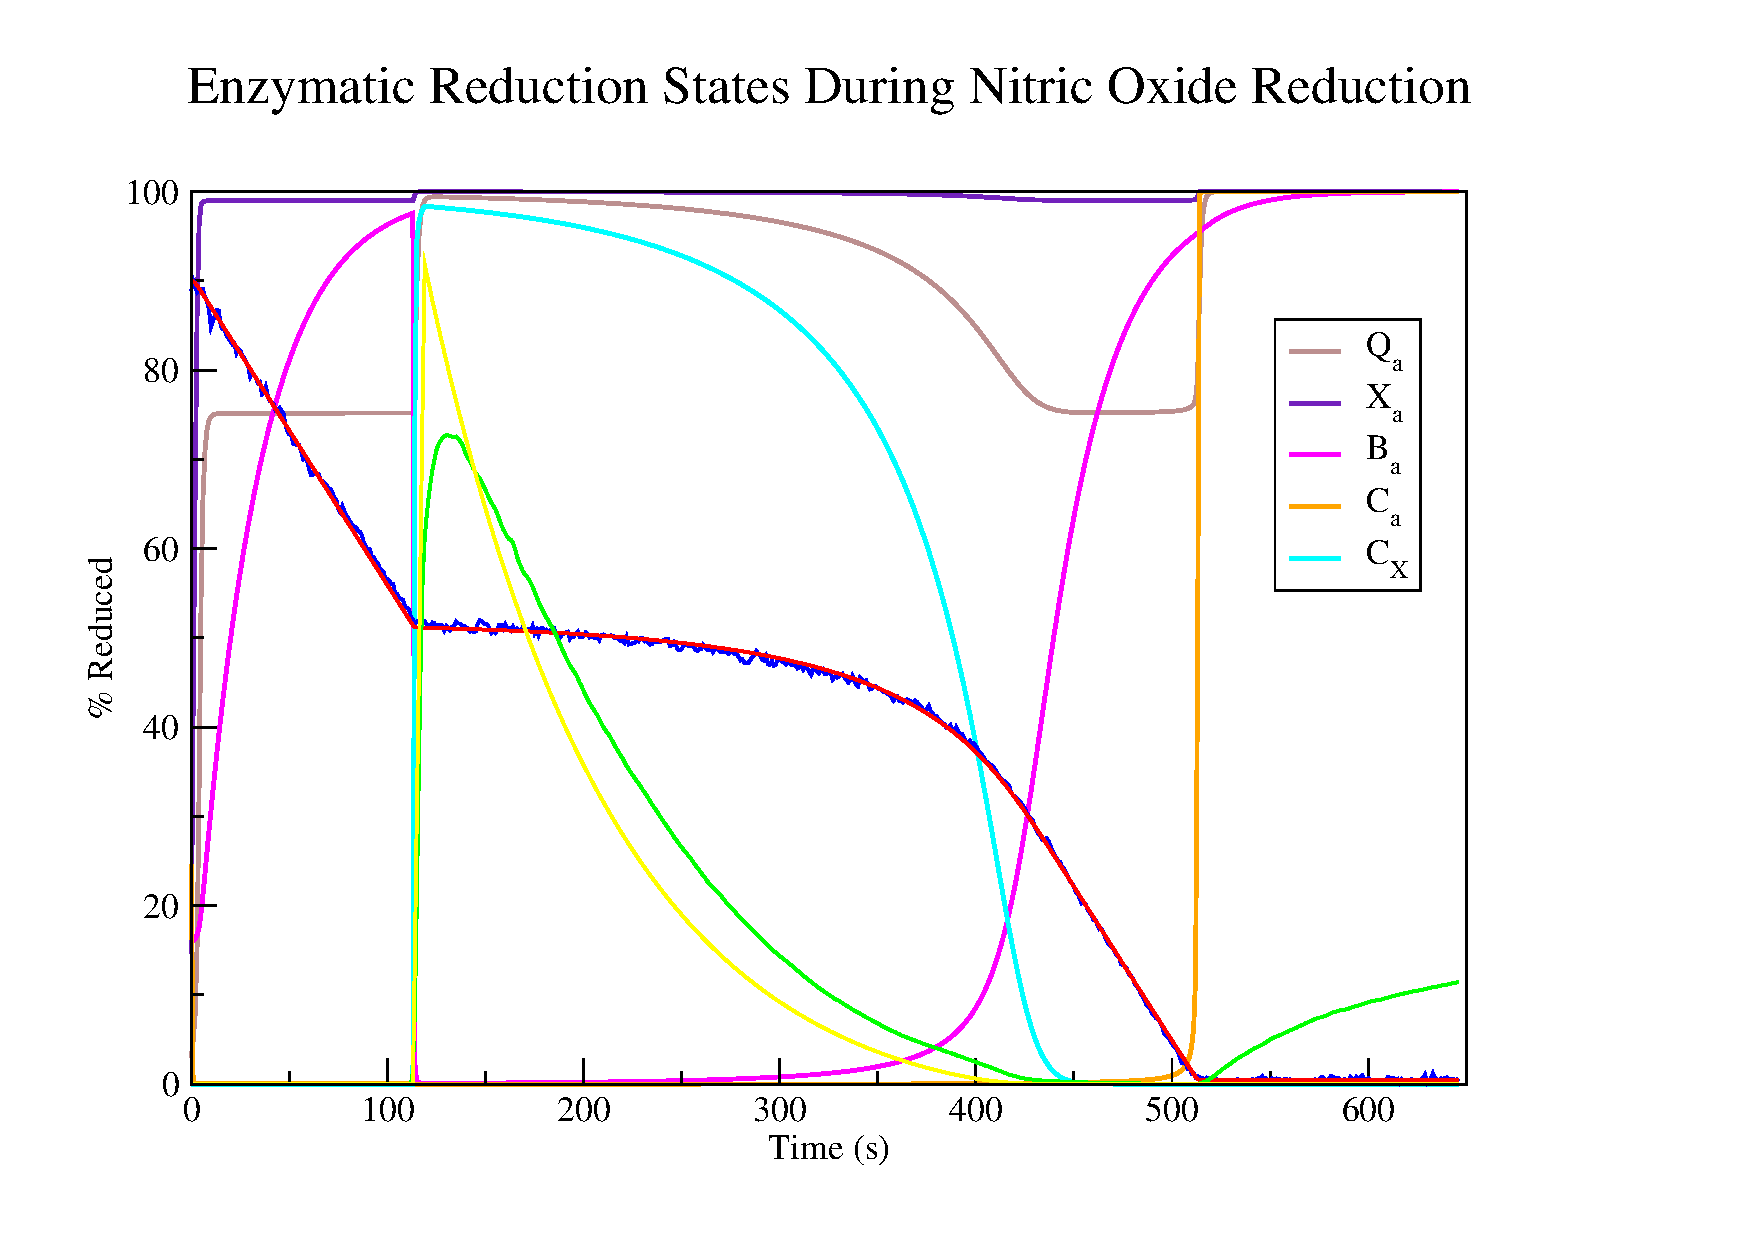
\includegraphics[width=15cm, trim=1cm 1cm 3cm 1cm, clip=true]{./06-noreduction/data/aer-no-sim-redox.pdf}
 % nosim.eps: 0x0 pixel, 300dpi, 0.00x0.00 cm, bb=0 0 794 595
 \caption[{Reduction States During Nitric Oxide Reduction.}]{{\bf Reduction States During Nitric Oxide Reduction.} This figure shows how the reduction states of the enzymes involved in respiration changes as the culture respires oxygen and then nitric oxide. The experimental and solved observed data are shown as thinner lines for reference.}
 \label{fig:nosimredox}
\end{figure}

%\section{Microaerobic Nitric Oxide Reduction}
%\subsection{Introduction}
%\subsection{Results}
%\subsection{Discussion}
\section{\texorpdfstring{Aerobic Nitric Oxide Reduction in \textit{nsrR$^\textrm{-}$} mutant}{Aerobic Nitric Oxide Reduction in nsrR- mutant}}
%\subsection{Introduction}
 The $\mathit{nsrR}^-$ mutant, which expresses NorB in an essentially constitutive manner was not effective in generating a usable dataset as it removed any NO almost instantaneously resulting in an almost featureless dataset (data not shown).
%\subsection{Results}
%\subsection{Discussion}